\chapter{粒子、场与相对论记号}

\section{课前的一个多普勒频移问题}

上周遗留的一个问题开启了讨论。一个以接近光速运动的观察者是否总是测得较长的波长？不：答案取决于运动方向。与光波同向运动的观察者看到其波长被拉长，而与光波逆向运动的观察者则看到其波长被压缩。这就是相对论性多普勒效应。

\begin{classroomqa}
\audiencequestion{接近光速的运动是否会使观测到的波长变长？}
\lecturerresponse{只有当观察者与光沿同一方向运动时才会如此。反转观察者的速度则反转频移的方向。这一结果可以直接由洛伦兹几何得到，无需记忆单独的公式。\lecturetimestamp{00:00:13}}
\end{classroomqa}

采用\(c=1\)的单位制，并令带撇系以速率\(v\)向右运动。一个向右运动的光波峰沿一条零线传播。将不带撇系的波长归一化为1，并把两个相继的波峰世界线写为
\begin{equation}
x=t,
\qquad
x=t+1.
\label{eq:sr5-crest-lines}
\end{equation}
不带撇系中的波长是在相等的\(t\)处测量两波峰之间的距离。而带撇系中的波长则必须在相等的\(t'\)处测量。因此，同时性的相对性就是整个计算的核心。

\begin{figure}[htbp]
\centering
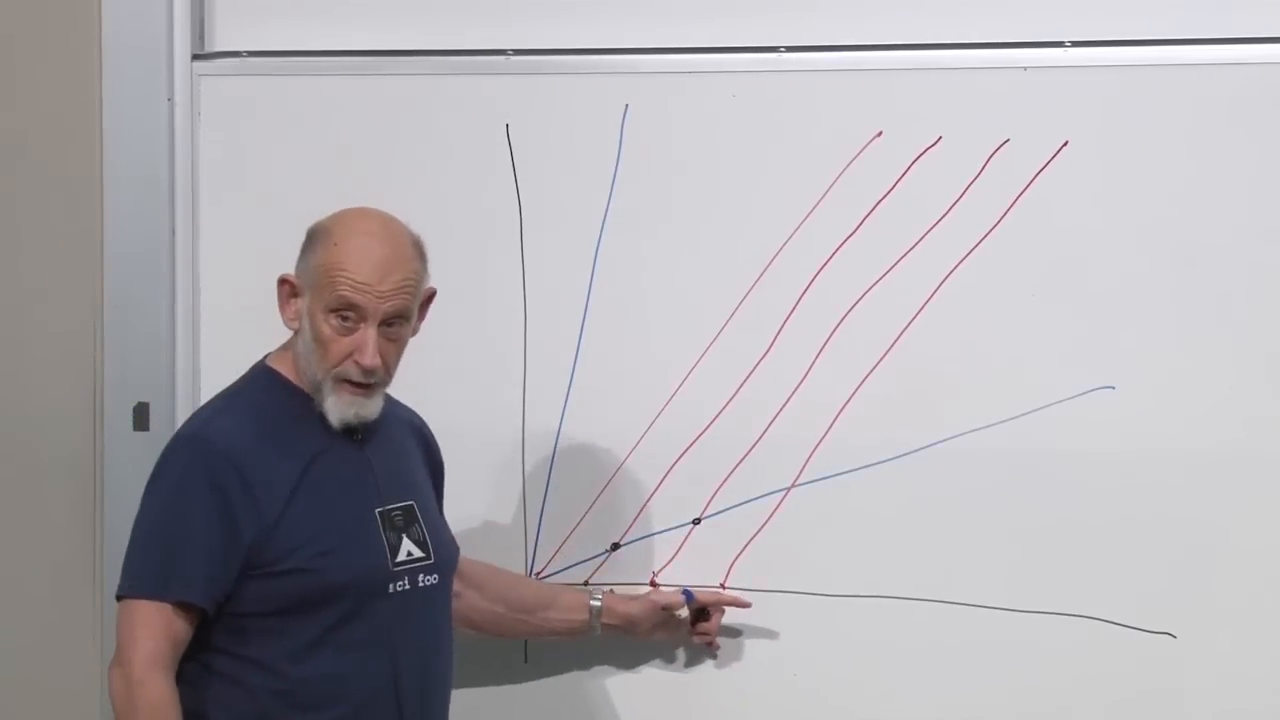
\includegraphics[width=0.90\textwidth]{lecture_05_figure_01.png}
\caption{相继的向右运动波峰、光锥以及运动系的倾斜坐标轴。}
\lectureframe{00:03:30}
\end{figure}

此时推导暂停，就课程顺序进行了简短讨论。将不会开设暑期课程。广义相对论以及更广泛地回归量子力学都是下一门课程的候选内容；谐振子被特别指出是在学习量子场论之前应当理解的内容。

\begin{classroomqa}
\audiencequestion{未来的课程能否讨论红外--紫外关联？}
\lecturerresponse{那个问题属于量子力学与引力的交汇处。本班所掌握的量子力学足以认识到这一问题，但必须先发展引力理论，最自然的途径是广义相对论。\lecturetimestamp{00:05:37}}
\end{classroomqa}

\begin{classroomqa}
\audiencequestion{倾斜坐标轴的相对尺度能否直接从黑板上的图读出？}
\lecturerresponse{不能。时空图记录的是因果性与同时性的几何结构，但在图上使用普通的欧几里得直尺并不是洛伦兹测量。应当定位相关事件并应用洛伦兹变换。\lecturetimestamp{00:06:10}}
\end{classroomqa}

现在恢复计算。将不带撇系的波峰间距归一化为1，并用代数方法定位带撇系中两个同时的事件。

洛伦兹变换为
\begin{equation}
t'=\gamma(t-vx),
\qquad
x'=\gamma(x-vt),
\qquad
\gamma=\frac{1}{\sqrt{1-v^2}}.
\label{eq:sr5-lorentz-doppler}
\end{equation}
选取带撇系的同时性切片\(t'=0\)。于是方程
\eqref{eq:sr5-lorentz-doppler}给出
\begin{equation}
t=vx.
\label{eq:sr5-primed-simultaneity}
\end{equation}
第一个波峰在原点与该切片相交。第二个波峰满足
\(x=t+1\)，因此其交点满足
\begin{align}
x&=vx+1,\\
x&=\frac{1}{1-v},
\qquad
t=\frac{v}{1-v}.
\end{align}
其带撇坐标为
\begin{align}
x'
&=\frac{x-vt}{\sqrt{1-v^2}}\\
&=\frac{1-v^2}{(1-v)\sqrt{1-v^2}}\\
&=\sqrt{\frac{1+v}{1-v}}.
\end{align}
由于原波长为1，
\begin{equation}
\boxed{
\frac{\lambda'}{\lambda}
=
\sqrt{\frac{1+\beta}{1-\beta}}
},
\qquad
\beta=\frac{v}{c}.
\label{eq:sr5-doppler}
\end{equation}
等价地，
\begin{equation}
\frac{\lambda'}{\lambda}
=
\sqrt{\frac{c+v}{c-v}}.
\end{equation}

\begin{figure}[htbp]
\centering
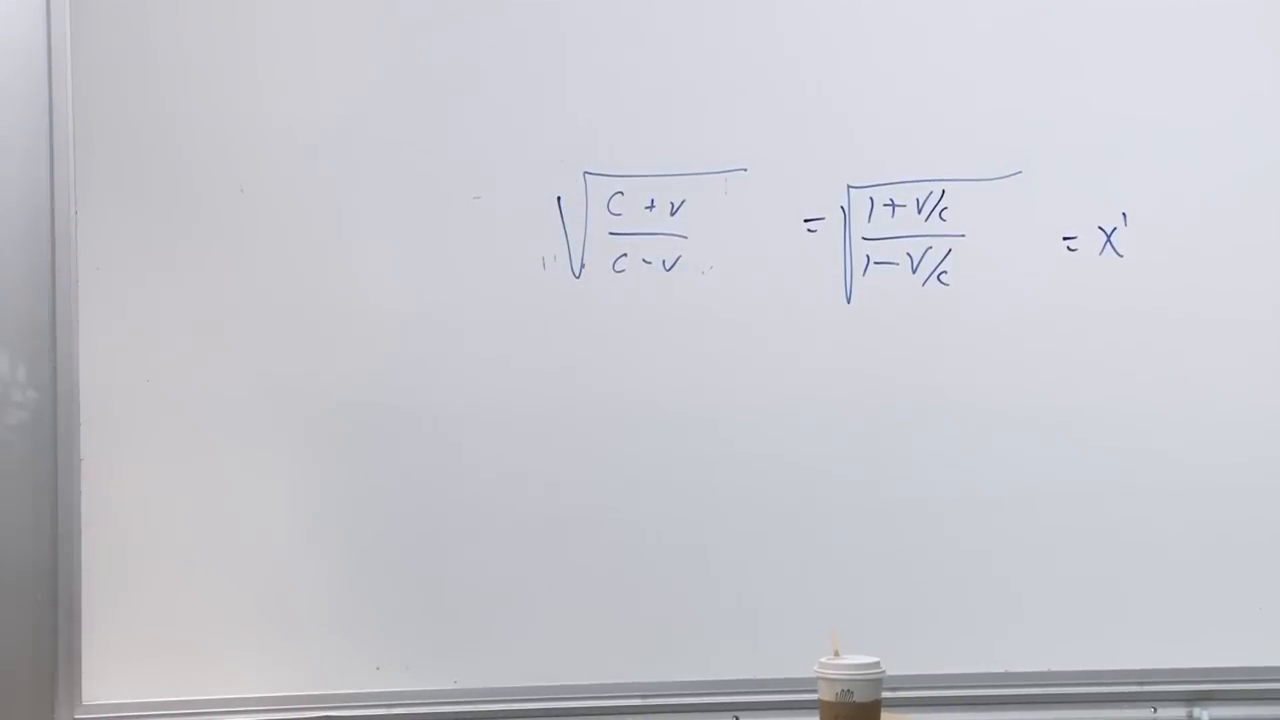
\includegraphics[width=0.90\textwidth]{lecture_05_figure_02.png}
\caption{恢复\(c\)后的多普勒因子；反转\(v\)则给出倒数频移。}
\lectureframe{00:13:40}
\end{figure}

对于\(v>0\)，带撇系的观察者追赶光并测得较长的波长。将\(v\)替换为\(-v\)则描述逆着光的运动，使该因子小于1。如果观察者在追赶光线的过程中能够趋近\(c\)，波长将发散。频率的移动则是其倒数比。

\section{为什么相互作用必须出现在同一个作用量中}

在预备问题之后，主题是场与粒子。在量子场论中，粒子与场最终将成为同一激发的两种描述。但这里的框架并非如此。在这里，粒子沿世界线运动，而经典场充满时空。当前的问题更为朴素：如果场作用于粒子，粒子又如何反过来作用于场？

作用量原理通过一个有限维的原型来回答这一问题。令\(x(t)\)和\(y(t)\)为两个广义坐标。如果拉格朗日量可分离，
\begin{equation}
L(x,\dot x,y,\dot y)
=
L_x(x,\dot x)+L_y(y,\dot y),
\label{eq:sr5-separable-l}
\end{equation}
那么两个欧拉--拉格朗日方程相互独立：
\begin{equation}
\frac{d}{dt}\frac{\partial L}{\partial\dot x}
=
\frac{\partial L}{\partial x},
\qquad
\frac{d}{dt}\frac{\partial L}{\partial\dot y}
=
\frac{\partial L}{\partial y}.
\end{equation}
\(x\)方程中不含\(y\)，而\(y\)方程中不含\(x\)。

为使这些变量发生相互作用，需添加一个无法拆分为\(x\)部分与\(y\)部分的项。一个简单的例子是
\begin{equation}
L
=
\frac{\dot x^2}{2}
+\frac{\dot y^2}{2}
-V(x)-W(y)+\kappa xy.
\label{eq:sr5-coupled-coordinates}
\end{equation}
现在，对\(x\)作变分会产生一个正比于\(y\)的项，而对\(y\)作变分则产生一个正比于\(x\)的项。同一个混合项支配着两个方向的影响。

\begin{figure}[htbp]
\centering
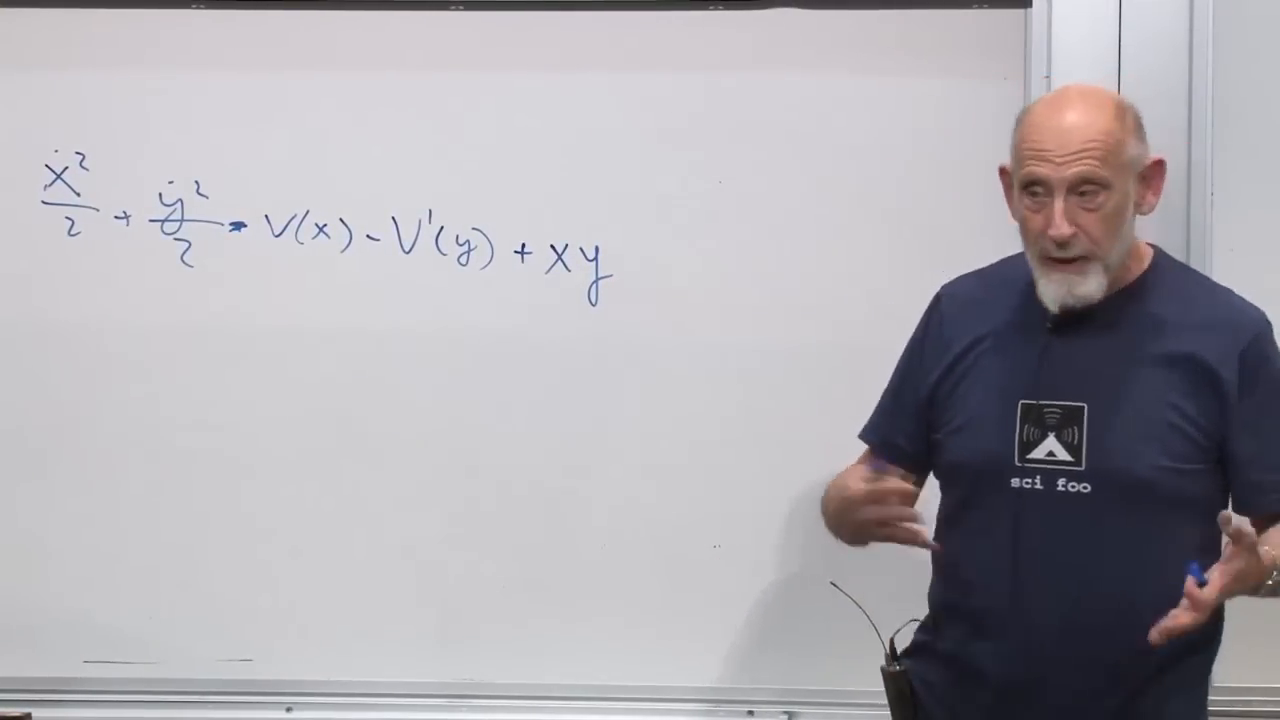
\includegraphics[width=0.90\textwidth]{lecture_05_figure_03.png}
\caption{当拉格朗日量中的某一项同时包含两个广义坐标时，这两个广义坐标便发生动力学耦合。}
\lectureframe{00:19:00}
\end{figure}

这就是此处所用作用--反作用表述的精确设定：两个对象都是动力学的，并且都在同一个共同作用中被变分。把场当作外部给定的背景来处理会掩盖它的响应，但一旦场本身是动力学的，耦合项就会同时给出两个方程。

\section{标量场如何作用于粒子}

\subsection{相对论性耦合}

首先把标量场\(\phi(\mathbf{x},t)\)视为已知的。它可以是波，也可以是静态分布；目前它自身的方程无关紧要。自由相对论性粒子的作用量为
\begin{equation}
S_{\mathrm p}
=
-m\int d\tau.
\end{equation}
对于直线上的运动且\(c=1\)，
\begin{equation}
L_{\mathrm p}^{(0)}
=
-m\sqrt{1-\dot x^2}.
\end{equation}
最简单的标量耦合把质量系数替换为依赖于场的系数：
\begin{equation}
\boxed{
L_{\mathrm p}
=
-\bigl[m+g\phi(x,t)\bigr]\sqrt{1-\dot x^2}
}.
\label{eq:sr5-particle-coupling}
\end{equation}
耦合常数\(g\)衡量场对该粒子影响的强度。它的符号是一种约定：把\(g\)改为\(-g\)会反转标量力的方向。

\begin{figure}[htbp]
\centering
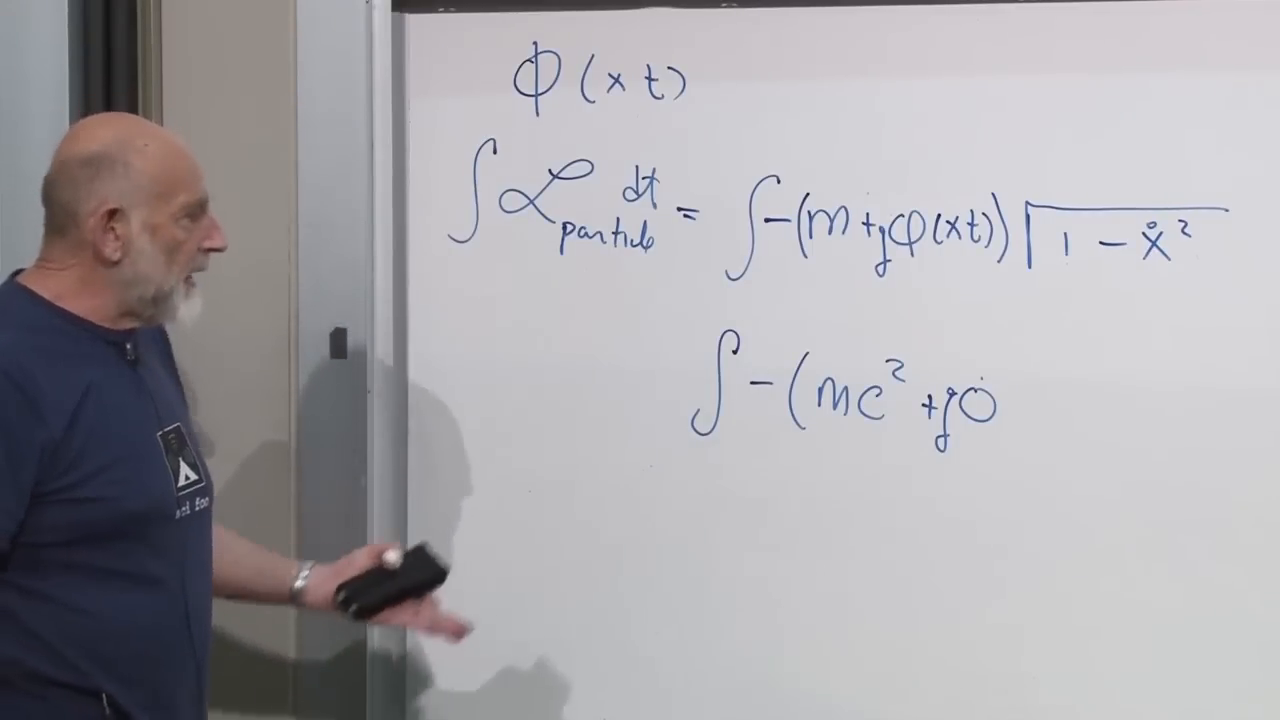
\includegraphics[width=0.90\textwidth]{lecture_05_figure_04.png}
\caption{将\(m\)替换为局域系数\(m+g\phi(x,t)\)后的自由粒子作用量。}
\lectureframe{00:24:10}
\end{figure}

\subsection{慢粒子极限}

恢复光速，使牛顿极限显现出来：
\begin{equation}
L_{\mathrm p}
=
-\bigl[mc^2+g\phi(x,t)\bigr]
\sqrt{1-\frac{\dot x^2}{c^2}}.
\label{eq:sr5-particle-coupling-c}
\end{equation}
对于\(|\dot x|\ll c\)，
\begin{equation}
\sqrt{1-\frac{\dot x^2}{c^2}}
=
1-\frac{\dot x^2}{2c^2}
+O\!\left(\frac{\dot x^4}{c^4}\right).
\end{equation}
代入\eqref{eq:sr5-particle-coupling-c}得到
\begin{align}
L_{\mathrm p}
&=
-mc^2-g\phi
+\frac{m\dot x^2}{2}
+\frac{g\phi\,\dot x^2}{2c^2}
+O(c^{-4})\\
&\longrightarrow
\frac{m\dot x^2}{2}-g\phi(x,t),
\label{eq:sr5-nr-particle}
\end{align}
其中已略去常数\(-mc^2\)以及被\(c^{-2}\)压低的项。结果就是通常的形式\(T-V\)，因此
\begin{equation}
V_{\mathrm p}(x,t)=g\phi(x,t).
\label{eq:sr5-scalar-potential}
\end{equation}

\begin{figure}[htbp]
\centering
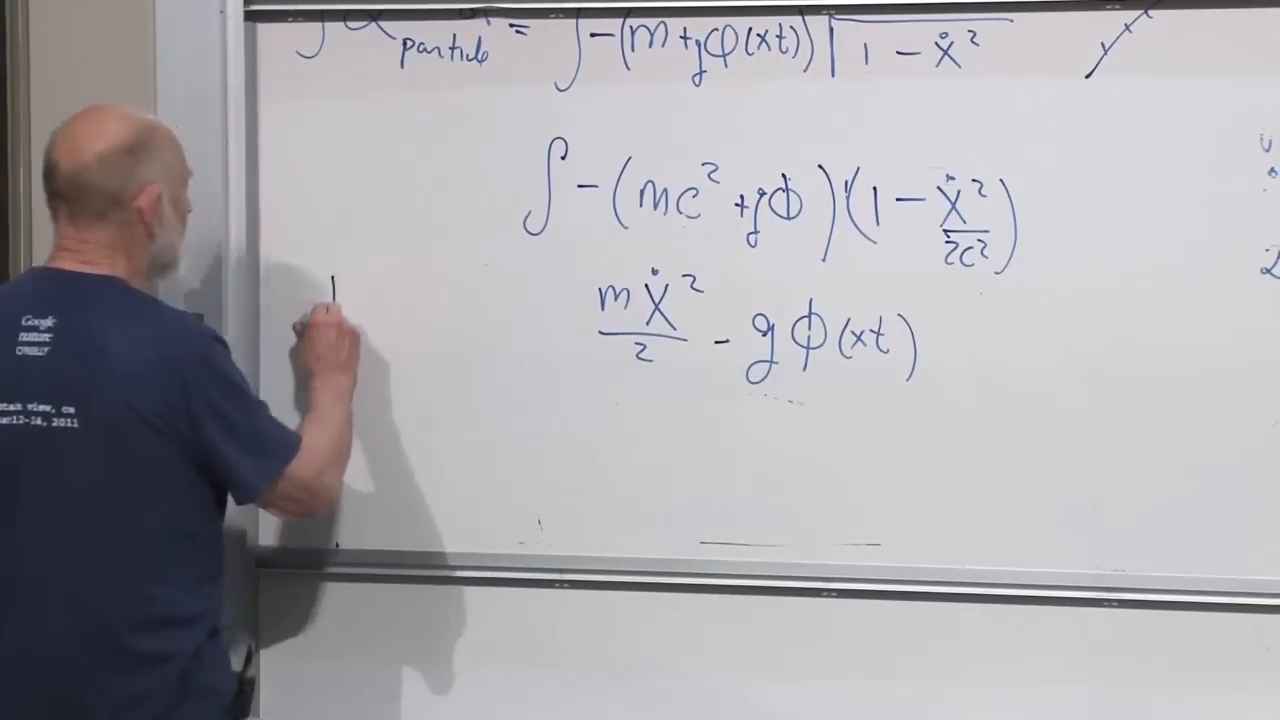
\includegraphics[width=0.90\textwidth]{lecture_05_figure_05.png}
\caption{平方根展开留下牛顿动能项和标量势能\(g\phi\)。}
\lectureframe{00:28:50}
\end{figure}

巨大的静止能量常数不进入欧拉--拉格朗日方程。依赖于场的项则进入。在电磁学中，电荷扮演着类似的耦合强度角色，尽管实际的电磁相互作用使用的是四维矢量势，而不是这个标量玩具模型。

\section{粒子如何反过来作用于场}

\subsection{一个变分问题}

场现在不能再仅仅是被给定的。考虑一个同时包含场位形和粒子世界线的时空区域。物理解使总作用量在对两者都变分时取驻值：
\begin{equation}
\delta S[\phi,x]=0.
\end{equation}
在保持场固定的同时变分世界线，给出粒子方程。在保持世界线固定的同时变分场，给出场方程。它们共同的相互作用项正是把两者联系起来的东西。

\begin{figure}[htbp]
\centering
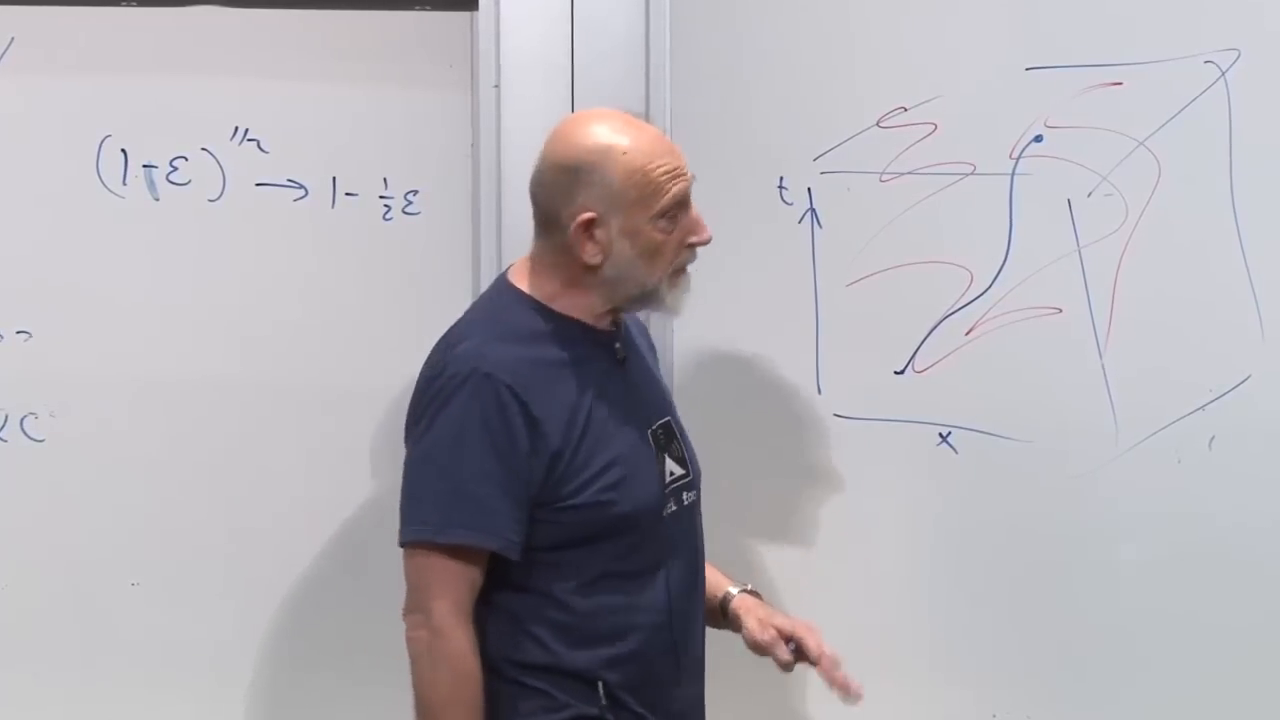
\includegraphics[width=0.90\textwidth]{lecture_05_figure_06.png}
\caption{一条粒子世界线穿过被标量场占据的时空区域。}
\lectureframe{00:30:30}
\end{figure}

对于自由无质量标量场，取
\begin{equation}
S_{\mathrm f}
=
\int d^4x\,
\frac12
\left[
(\partial_t\phi)^2
-(\partial_x\phi)^2
-(\partial_y\phi)^2
-(\partial_z\phi)^2
\right].
\label{eq:sr5-free-field-action}
\end{equation}
从此刻起，再次使用\(c=1\)。若写出显式单位，时间项将带有相应的\(1/c^2\)因子，具体取决于坐标和场的归一化。

\begin{figure}[htbp]
\centering
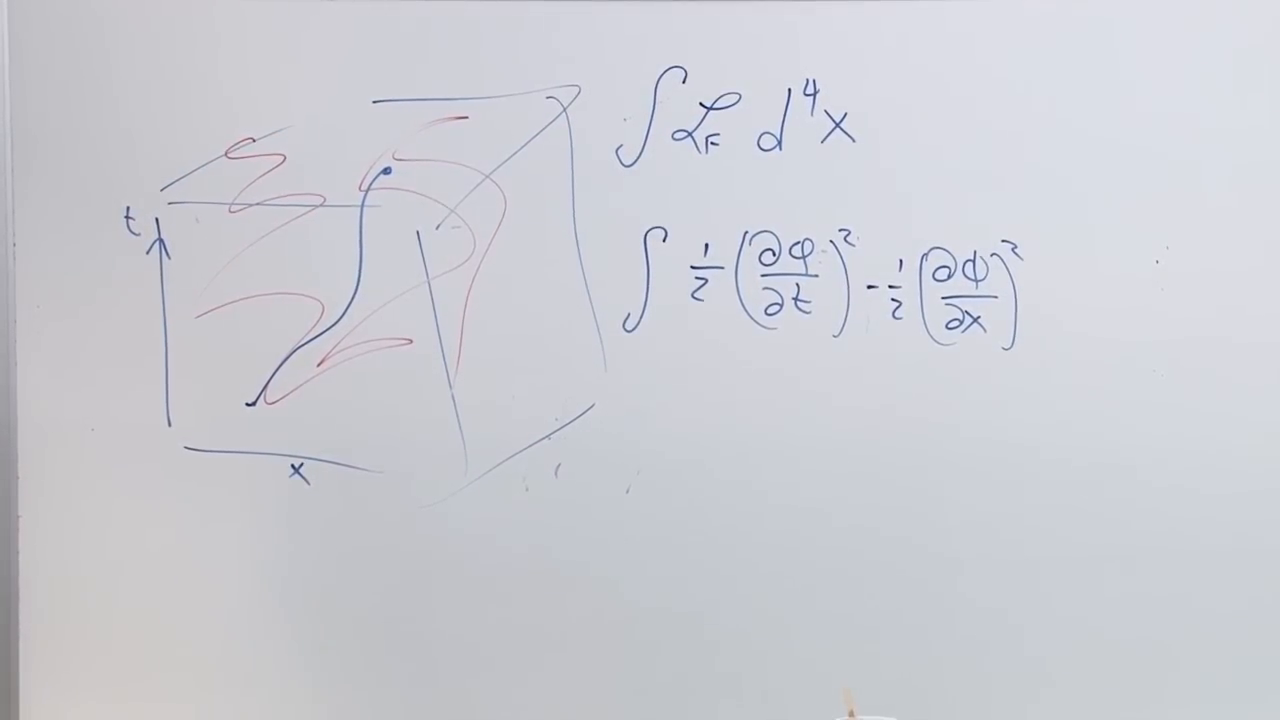
\includegraphics[width=0.90\textwidth]{lecture_05_figure_07.png}
\caption{在与粒子世界线相同的时空区域上写出的场作用量。}
\lectureframe{00:32:10}
\end{figure}

\subsection{静态粒子与世界线积分}

为了以最少的代数运算暴露出源，把粒子静止放在原点。因子\(d\tau\)于是等于\(dt\)，而\eqref{eq:sr5-particle-coupling}的相互作用部分变为
\begin{equation}
S_{\mathrm{int}}
=
-g\int dt\,\phi(\mathbf{0},t).
\label{eq:sr5-worldline-interaction}
\end{equation}
这只是一个沿世界线的积分，而
\eqref{eq:sr5-free-field-action}是对整个时空的积分。要把它们合并成一个时空积分，我们需要一个能选出粒子位置的函数。

\begin{figure}[htbp]
\centering
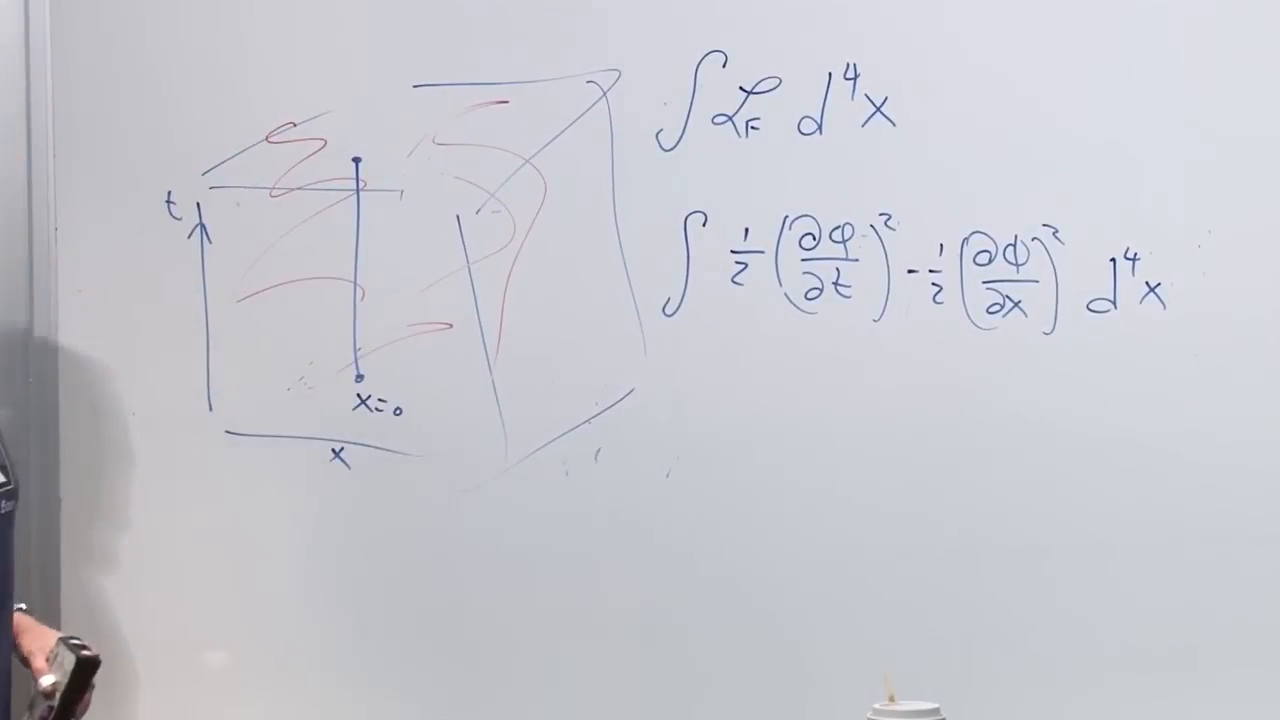
\includegraphics[width=0.90\textwidth]{lecture_05_figure_08.png}
\caption{场区域内的静态世界线以及必须与之合并的场作用量。}
\lectureframe{00:35:35}
\end{figure}

\subsection{狄拉克{\proseunicodefont δ}函数}

一维{\proseunicodefont δ}函数由下式定义
\begin{equation}
\int_{-\infty}^{\infty}dx\,f(x)\delta(x-a)=f(a).
\label{eq:sr5-delta-definition}
\end{equation}
它在\(x=a\)之外为零，在\(x=a\)处奇异，并且积分为单位值。最好把它理解为一个由
\eqref{eq:sr5-delta-definition}刻画的分布，而不是一个普通的取有限值的函数。

\begin{figure}[htbp]
\centering
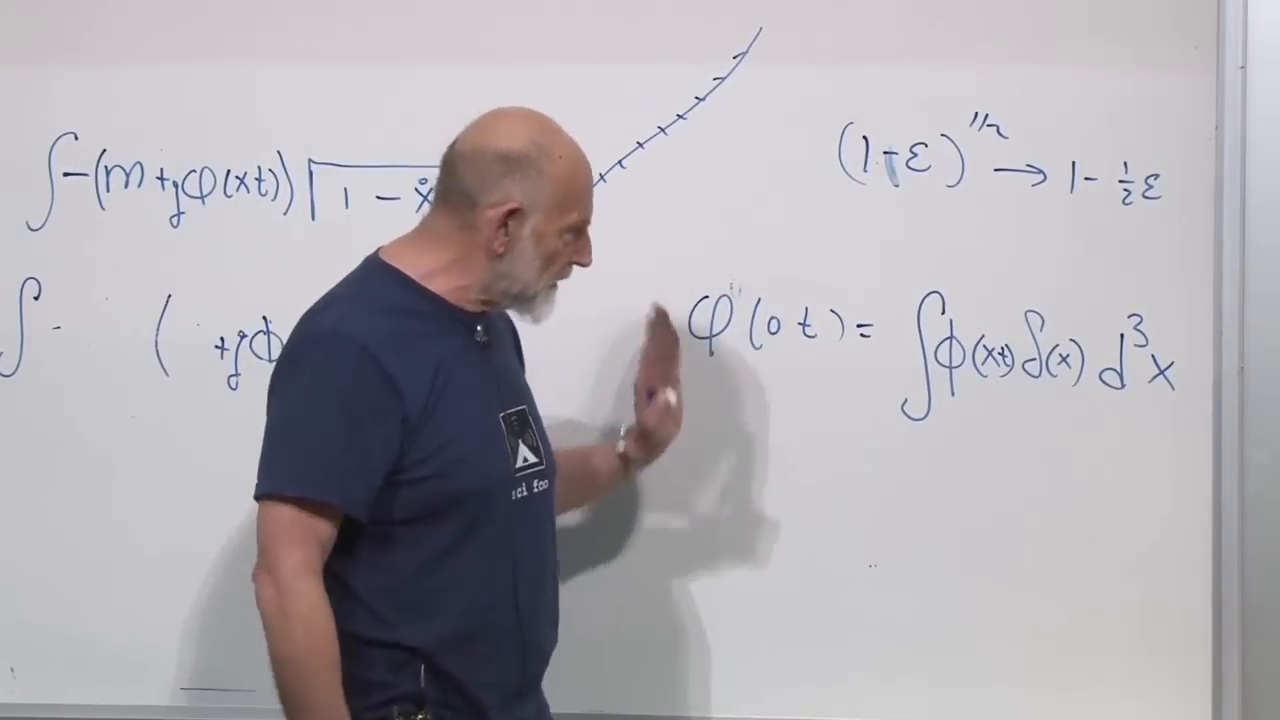
\includegraphics[width=0.90\textwidth]{lecture_05_figure_09.png}
\caption{把原点处的场值改写为空间积分的{\proseunicodefont δ}函数恒等式。}
\lectureframe{00:36:45}
\end{figure}

在三维中，
\begin{equation}
\delta^3(\mathbf{x})
=
\delta(x)\delta(y)\delta(z),
\end{equation}
因此
\begin{align}
\int d^3x\,
\phi(\mathbf{x},t)\delta^3(\mathbf{x})
&=
\int dx\,dy\,dz\,
\phi(x,y,z,t)\\
&\quad\times\delta(x)\delta(y)\delta(z)\\
&=\phi(\mathbf{0},t).
\label{eq:sr5-triple-delta}
\end{align}

\begin{classroomqa}
\audiencequestion{\(d^3x\)从何而来？}
\lecturerresponse{它就是通常的空间体积元\(dx\,dy\,dz\)。在一维空间中，同一恒等式只包含\(dx\)和一个{\proseunicodefont δ}函数。\lecturetimestamp{00:37:09}}
\end{classroomqa}

\begin{figure}[htbp]
\centering
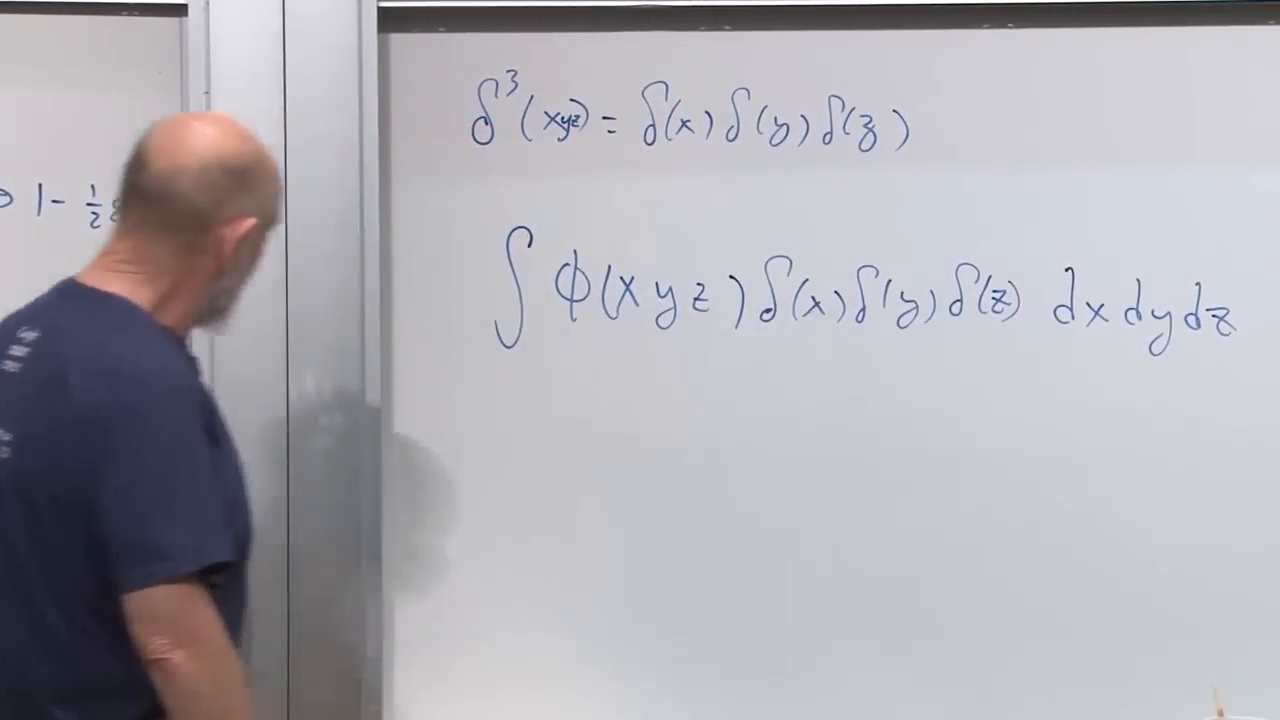
\includegraphics[width=0.90\textwidth]{lecture_05_figure_10.png}
\caption{三维{\proseunicodefont δ}函数展开为三个一维因子。}
\lectureframe{00:39:05}
\end{figure}

方程 \eqref{eq:sr5-worldline-interaction} 现在可以写成
\begin{equation}
S_{\mathrm{int}}
=
-g\int d^4x\,
\delta^3(\mathbf{x})\phi(\mathbf{x},t).
\end{equation}
完整的静态源作用量为
\begin{align}
S
=
\int d^4x
\biggl\{
&\frac12(\partial_t\phi)^2
-\frac12|\boldsymbol{\nabla}\phi|^2
\nonumber\\
&-g\delta^3(\mathbf{x})\phi
\biggr\}.
\label{eq:sr5-combined-action}
\end{align}

\begin{classroomqa}
\audiencequestion{将相互作用插入时空作用量时，是否丢掉了一个负号？}
\lecturerresponse{世界线拉格朗日量包含 \(-g\phi\)，因此时空密度必须包含 \(-g\delta^3(\mathbf{x})\phi\)。保持该符号即可确定场方程中的源项。\lecturetimestamp{00:41:24}}
\end{classroomqa}

\begin{figure}[htbp]
\centering
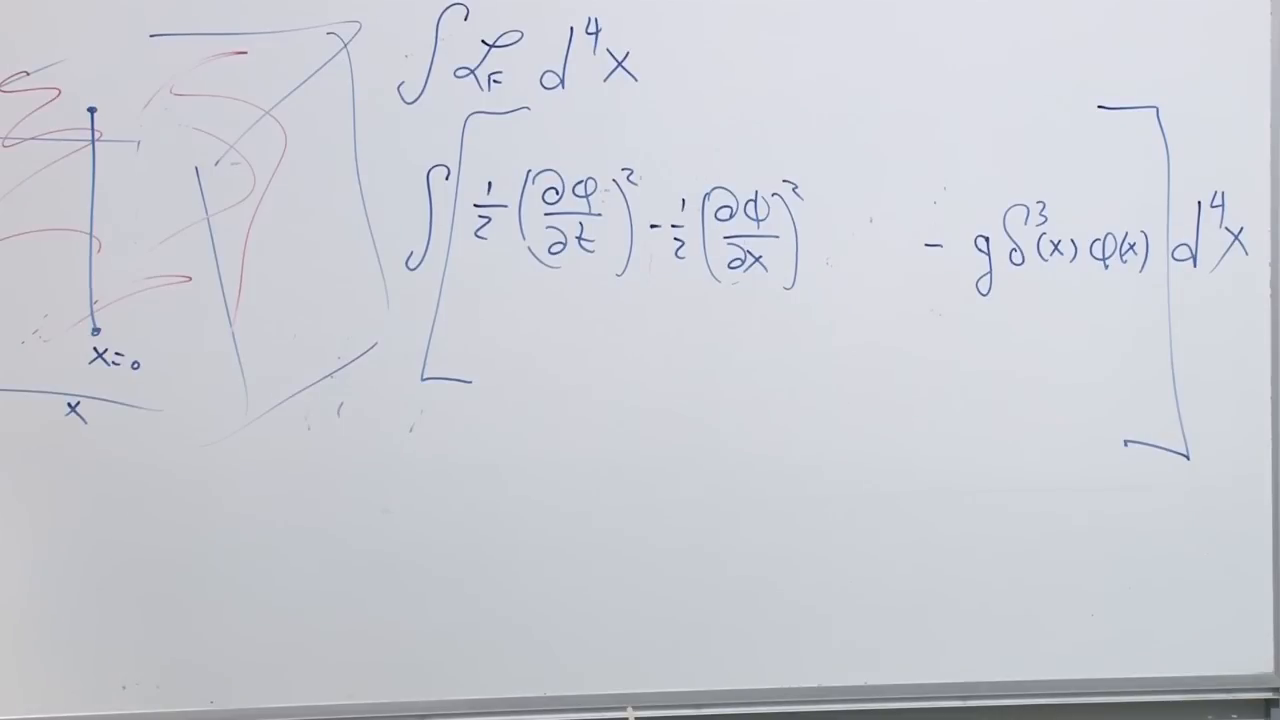
\includegraphics[width=0.90\textwidth]{lecture_05_figure_11.png}
\caption{自由标量密度与局域相互作用被组装成一个时空作用量。}
\lectureframe{00:42:05}
\end{figure}

\subsection{有源场方程}

对 \eqref{eq:sr5-combined-action} 关于 \(\phi\) 变分，得到
\begin{equation}
\boxed{
\partial_t^2\phi-\nabla^2\phi
=
-g\delta^3(\mathbf{x})
}.
\label{eq:sr5-sourced-wave}
\end{equation}
在原点之外，这就是自由波动方程。在原点处，delta 函数将粒子标记为局域源。

\begin{figure}[htbp]
\centering
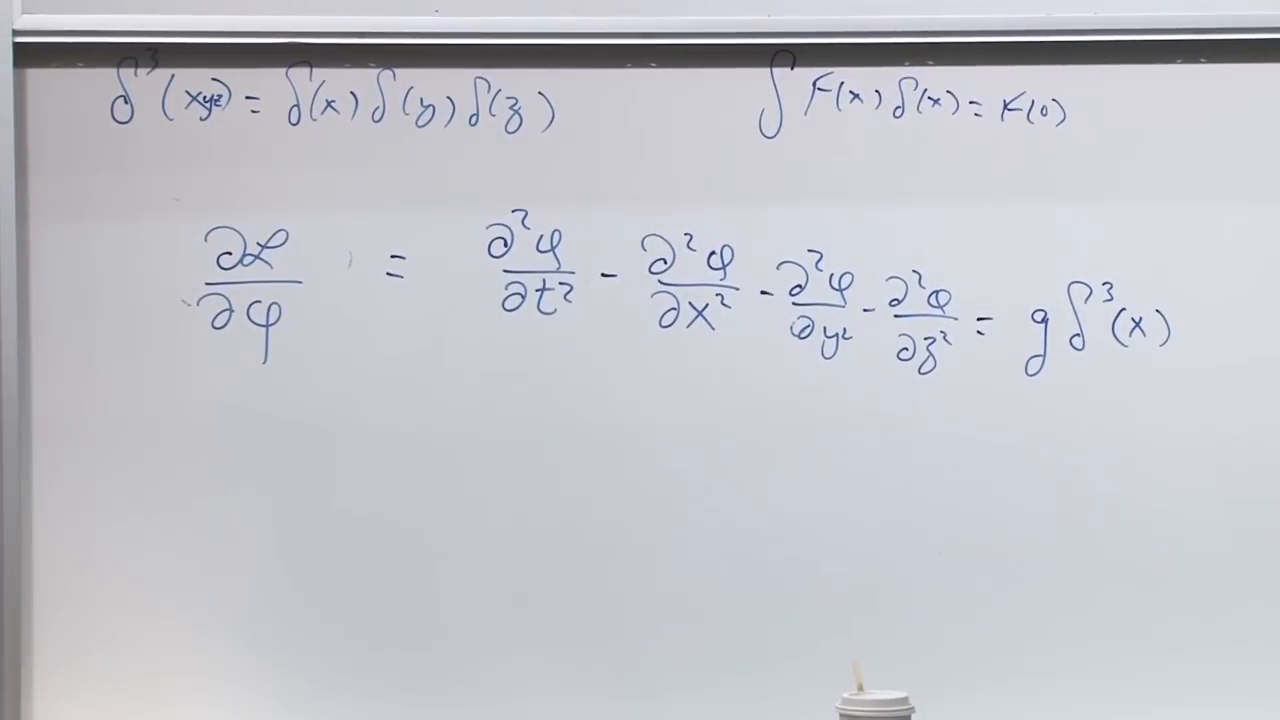
\includegraphics[width=0.90\textwidth]{lecture_05_figure_12.png}
\caption{由原点处点源驱动的波动算子。}
\lectureframe{00:45:35}
\end{figure}

对于静态解，\(\partial_t\phi=0\)，因此
\begin{equation}
\boxed{
\nabla^2\phi
=
g\delta^3(\mathbf{x})
}.
\label{eq:sr5-poisson}
\end{equation}
这是点源的泊松方程。这里的类比是静电的，还不是电磁的：场仍然是标量 \(\phi\)，而不是电磁四维势。

\begin{figure}[htbp]
\centering
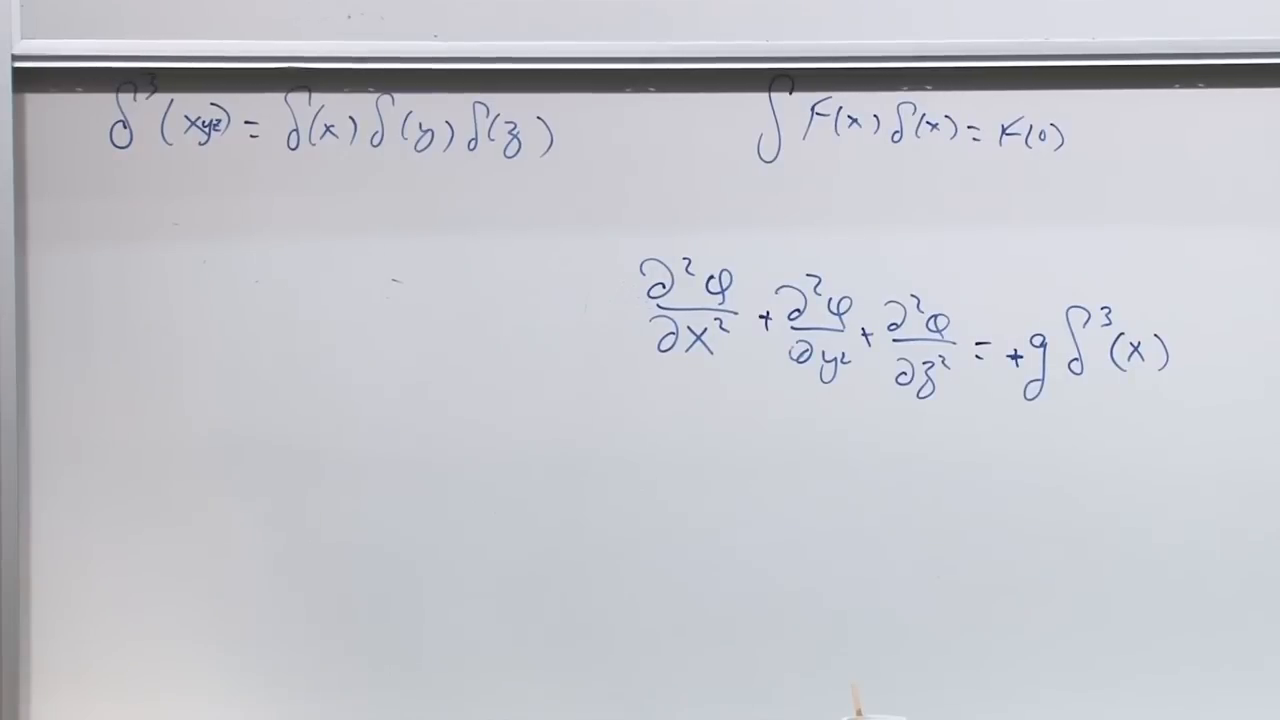
\includegraphics[width=0.90\textwidth]{lecture_05_figure_13.png}
\caption{有源波动方程的静态极限，可辨认为泊松方程。}
\lectureframe{00:47:05}
\end{figure}

这种互易性现在已明确显现。项 \(g\phi\) 赋予粒子势能，而同一个 \(g\) 又使该粒子成为 \(\phi\) 的源。这两种效应并非彼此独立的假设。

\subsection{运动源会辐射}

固定在 \(\mathbf{a}\) 处的粒子由
\(\delta^3(\mathbf{x}-\mathbf{a})\) 表示。如果它的位置随时间变化，源就变为
\begin{equation}
\delta^3\!\left(\mathbf{x}-\mathbf{a}(t)\right).
\label{eq:sr5-moving-delta}
\end{equation}
含时的右端项无法由不含时的场来平衡。\(\partial_t^2\phi\) 项必须重新出现，而加速或振荡的源可以向场中发射波。

\begin{figure}[htbp]
\centering
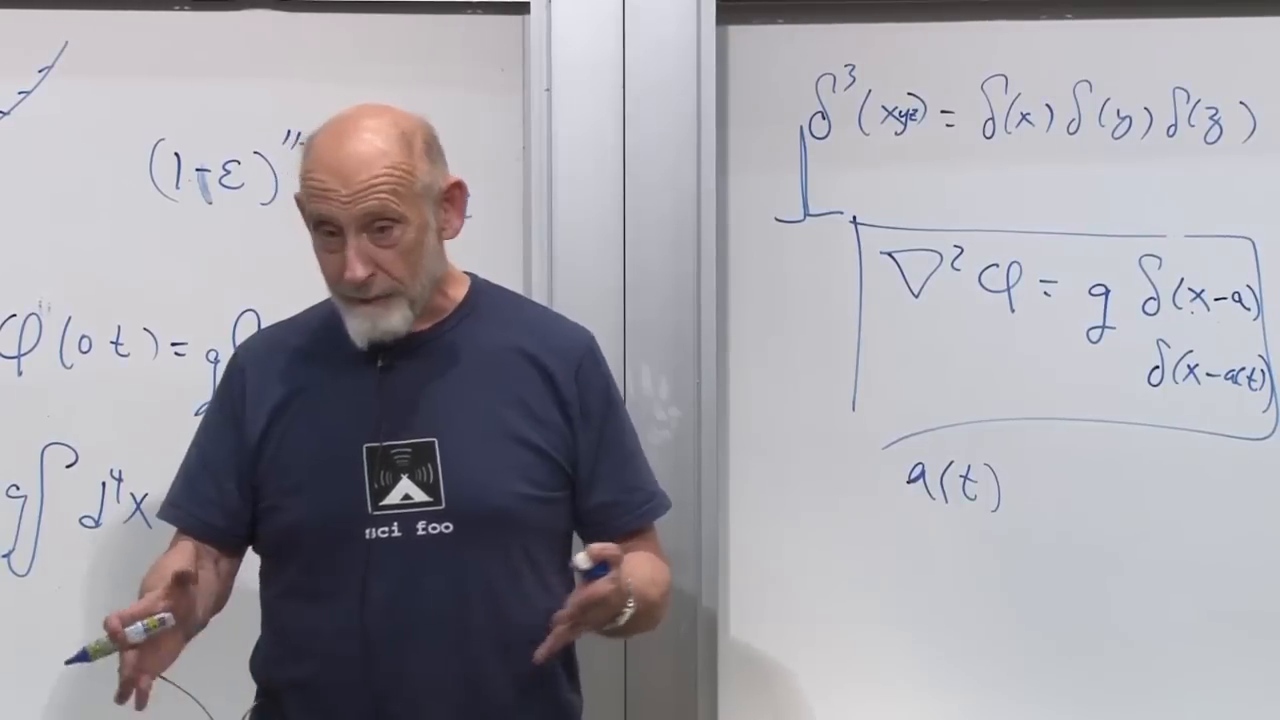
\includegraphics[width=0.90\textwidth]{lecture_05_figure_14.png}
\caption{一个平移到 \(\mathbf{a}(t)\) 的 delta 函数源，使场方程成为含时的。}
\lectureframe{00:50:30}
\end{figure}

\begin{classroomqa}
\audiencequestion{如果源按非相对论方式处理，那么场方程中的相对论性在哪里？}
\lecturerresponse{相对论性传播被编码在左侧的时空波动算子中。完全相对论性的粒子处理会保留其固有时作用量和速度因子。即使缓慢运动但含时的源也能驱动波。\lecturetimestamp{00:52:14}}
\end{classroomqa}

\begin{classroomqa}
\audiencequestion{\(g\phi\) 必须具有什么单位？}
\lecturerresponse{它在粒子作用量中与 \(mc^2\) 并列出现，因此具有能量的单位。在这里使用的自然单位归一化下，\(3+1\) 维中的标量具有质量量纲一，而 \(g\) 可以是无量纲的。量纲会随时空维数和场归一化而改变。\lecturetimestamp{00:52:55}}
\end{classroomqa}

\section{四维矢量、标量与度规}

分量方程已经变得足够长，因此有必要采用更好的记号。将时空坐标写成
\begin{equation}
x^\mu=(x^0,x^1,x^2,x^3)=(t,x,y,z),
\label{eq:sr5-four-coordinate}
\end{equation}
其中希腊指标遍历全部四个分量。一个四分量列表并不自动就是四维矢量。只有当其分量在洛伦兹变换下的变换方式与 \(x^\mu\) 相同时，它才是四维矢量。

\begin{figure}[htbp]
\centering
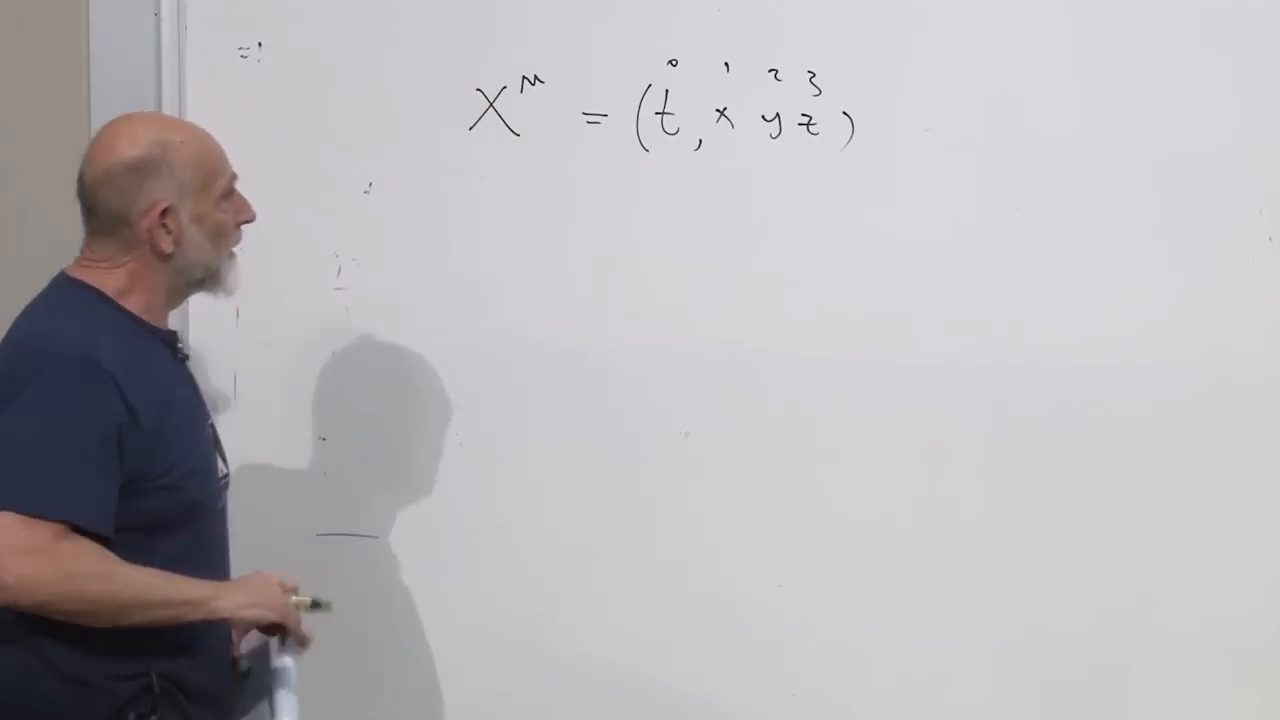
\includegraphics[width=0.90\textwidth]{lecture_05_figure_15.png}
\caption{四个时空坐标被汇集为 \(x^\mu\)。}
\lectureframe{00:55:00}
\end{figure}

关于三个空间分量消失的陈述可能在一个参考系中成立，而在另一个参考系中不成立。相比之下，如果全部四个分量都消失，那么每个洛伦兹观察者都会同意该矢量为零。诸如 \(dx^\mu\) 这样的差值也是四维矢量。

不变固有时区间为
\begin{equation}
d\tau^2
=
dt^2-dx^2-dy^2-dz^2.
\label{eq:sr5-proper-time}
\end{equation}
它只有一个值，而不是四个依赖于参考系的分量，因此它是一个标量。

\begin{figure}[htbp]
\centering
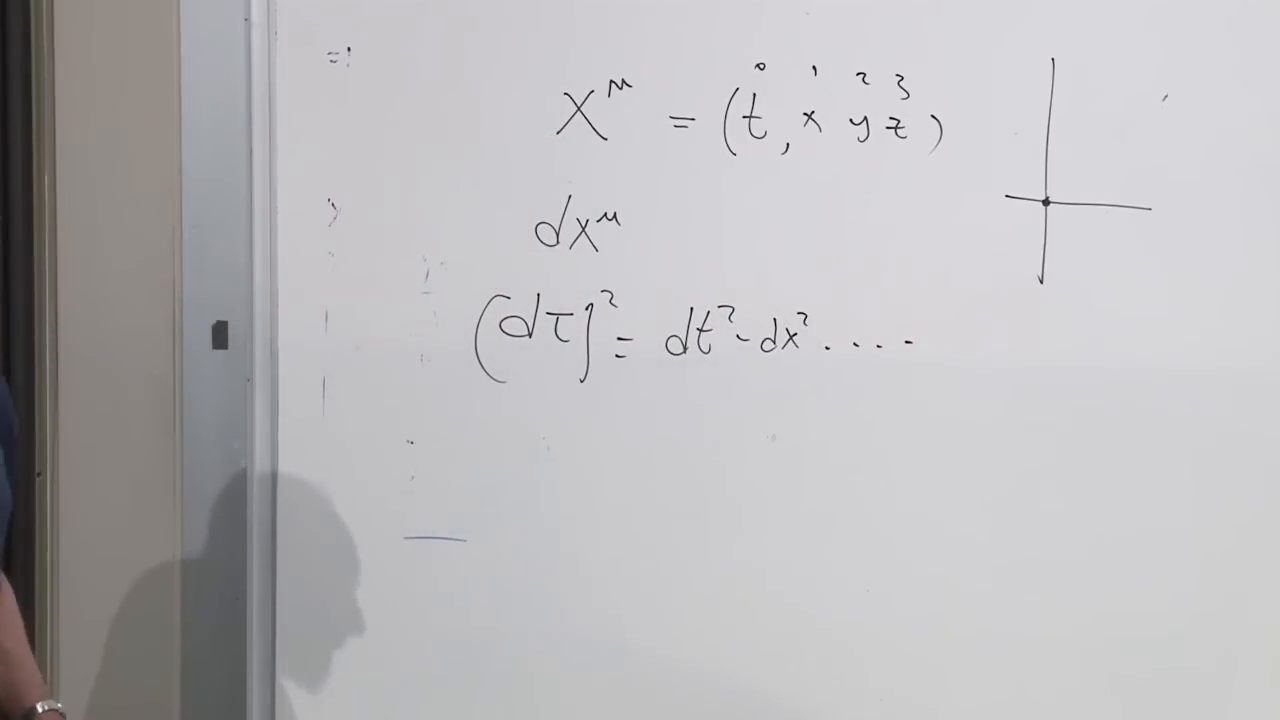
\includegraphics[width=0.90\textwidth]{lecture_05_figure_16.png}
\caption{四维位移与不变固有时区间。}
\lectureframe{00:57:25}
\end{figure}

\subsection{闵可夫斯基度规}

采用 mostly-plus 号差
\begin{equation}
\eta_{\mu\nu}
=
\operatorname{diag}(-1,1,1,1).
\label{eq:sr5-metric}
\end{equation}
另一种 mostly-minus 约定同样有效，但每个方程都必须一致地使用一种约定。采用 \eqref{eq:sr5-metric} 时，
\begin{equation}
dx^\mu dx_\mu
=
-dt^2+dx^2+dy^2+dz^2
=
-d\tau^2.
\end{equation}
整体符号不会改变不变性。

\begin{figure}[htbp]
\centering
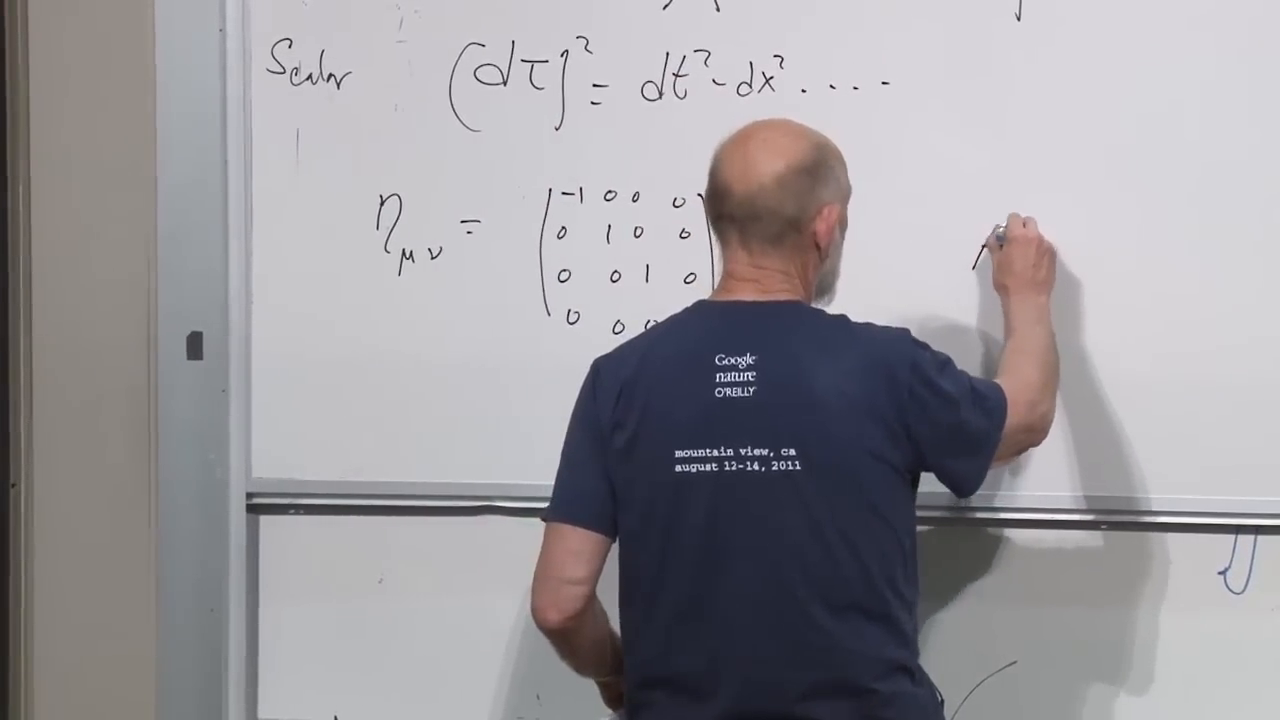
\includegraphics[width=0.90\textwidth]{lecture_05_figure_17.png}
\caption{写成对角矩阵的 mostly-plus 闵可夫斯基度规。}
\lectureframe{01:00:30}
\end{figure}

度规降低一个指标：
\begin{equation}
A_\mu=\eta_{\mu\nu}A^\nu.
\label{eq:sr5-lower-index}
\end{equation}
对于这个笛卡儿度规，
\begin{equation}
A^\mu=(A^0,A^1,A^2,A^3),
\qquad
A_\mu=(-A^0,A^1,A^2,A^3).
\label{eq:sr5-upper-lower-components}
\end{equation}
再次应用同一个度规会升高指标，因为
\(\eta^{\mu\rho}\eta_{\rho\nu}=\delta^\mu{}_\nu\)。

\begin{figure}[htbp]
\centering
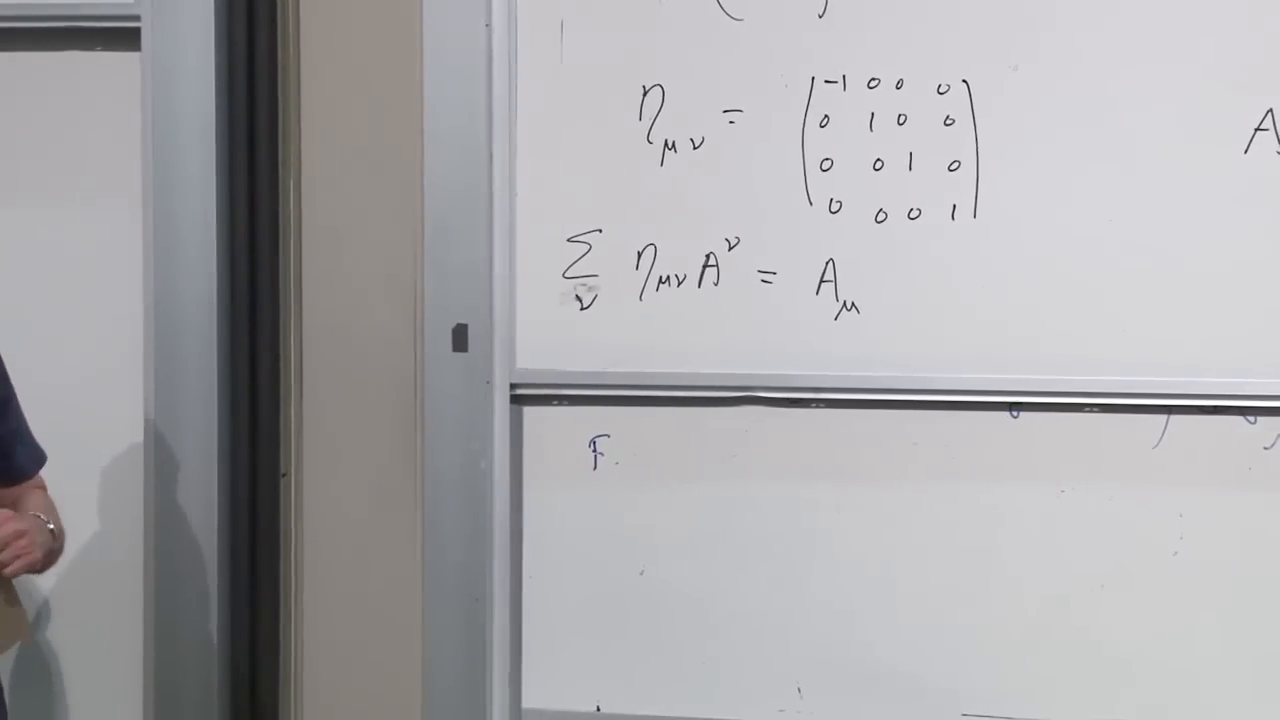
\includegraphics[width=0.90\textwidth]{lecture_05_figure_18.png}
\caption{通过乘以 \(\eta_{\mu\nu}\) 的矩阵乘法来降低指标。}
\lectureframe{01:03:00}
\end{figure}

\begin{classroomqa}
\audiencequestion{普通的矩阵乘法在这里真的包含一个求和吗？}
\lecturerresponse{是的。每个输出分量都是\(\eta\)的一行乘以整个向量：即对列指标求和。对角度规使计算看起来很简单，但一般矩阵会使这个求和明确显现。\lecturetimestamp{01:04:56}}
\end{classroomqa}

\subsection{爱因斯坦求和约定与自由指标}

爱因斯坦约定规定，只要一个指标在上方出现一次、在下方出现一次，就省略求和符号：
\begin{equation}
\eta_{\mu\nu}A^\nu
\equiv
\sum_{\nu=0}^{3}\eta_{\mu\nu}A^\nu.
\end{equation}
这里\(\nu\)是哑指标；它被求和掉，可以重新命名。指标\(\mu\)是自由的，标记结果的四个分量。一个指标通常不应在一个单项式中出现超过两次。

传统的名称是：上指标称为\emph{逆变}，下指标称为\emph{协变}。本讲有意更倾向于使用更朴素的说法\emph{上}和\emph{下}，但两种术语指的都是相同的变换规则。

\section{标量的缩并与导数}

\subsection{闵可夫斯基内积}

将一个向量与其降指标形式缩并，得到
\begin{equation}
A^\mu A_\mu
=
\eta_{\mu\nu}A^\mu A^\nu
=
-(A^0)^2+(A^1)^2+(A^2)^2+(A^3)^2.
\label{eq:sr5-vector-square}
\end{equation}
不应手动插入额外的负号；它已经来自降指标后的时间分量。

\begin{figure}[htbp]
\centering
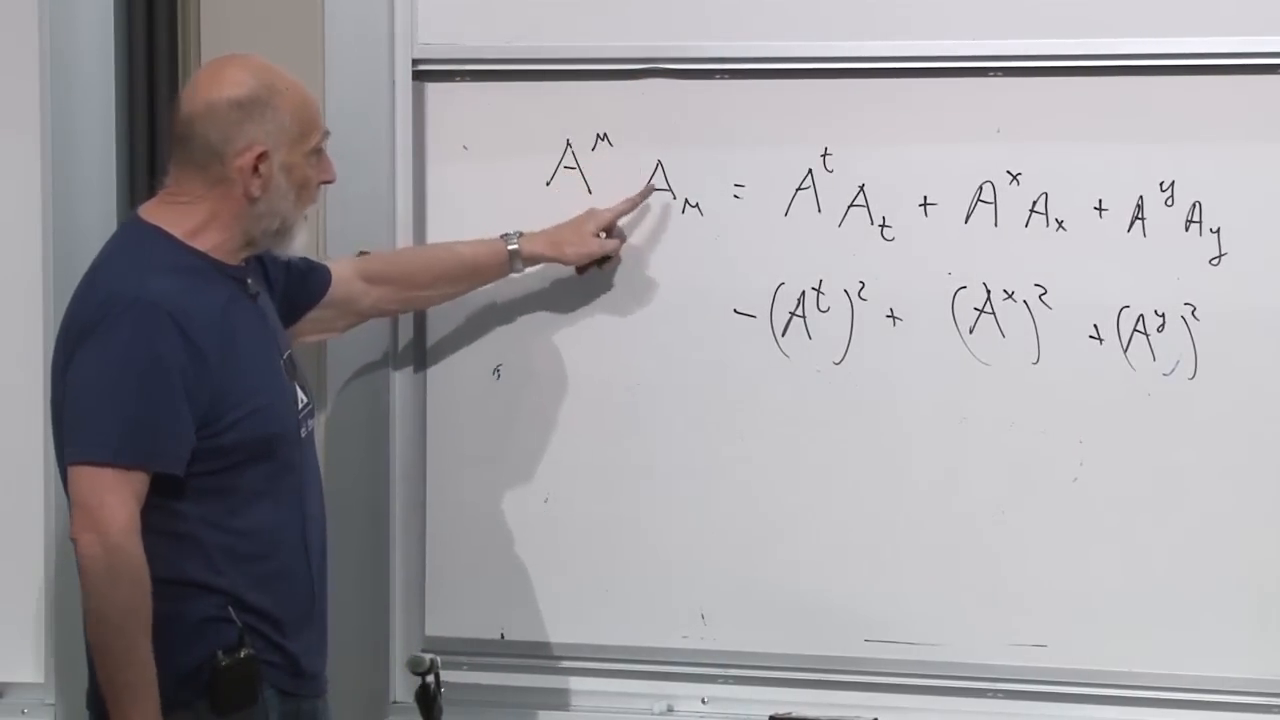
\includegraphics[width=0.90\textwidth]{lecture_05_figure_19.png}
\caption{缩并\(A^\mu A_\mu\)展开为时间分量和空间分量。}
\lectureframe{01:09:30}
\end{figure}

\begin{classroomqa}
\audiencequestion{下指标向量应该画成行而不是列吗？}
\lecturerresponse{在初等矩阵记号中，它可以表示成一行，但指标记号并不要求这种选择。它的定义性特征是它如何变换，以及它如何与上指标向量缩并。\lecturetimestamp{01:10:26}}
\end{classroomqa}

\begin{classroomqa}
\audiencequestion{希腊指标总是指全部四个分量吗？}
\lecturerresponse{在这种记号中，是的。诸如\(\mu,\nu\)这样的希腊指标遍历时空，而诸如\(i,j\)这样的拉丁指标通常只遍历三个空间分量。\lecturetimestamp{01:12:23}}
\end{classroomqa}

同样的构造对两个不同的四维向量也成立：
\begin{equation}
A^\mu B_\mu
\end{equation}
是一个标量。一个简短的证明使用极化恒等式。由于
\((A+B)^2\)和\((A-B)^2\)都是标量，
\begin{equation}
(A+B)^2-(A-B)^2=4A^\mu B_\mu
\end{equation}
也是标量。这是普通点积的闵可夫斯基版本。

\begin{classroomqa}
\audiencequestion{\(A^\mu B_\mu\)是否类似于普通点积？}
\lecturerresponse{完全正确，只不过闵可夫斯基度规提供了时间分量与空间分量之间的相对符号。\lecturetimestamp{01:15:44}}
\end{classroomqa}

\subsection{梯度是一个余向量}

设\(\phi(x)\)为一个标量场，其中\(x\)现在代表全部四个时空坐标。在相邻事件之间，
\begin{equation}
d\phi
=
\frac{\partial\phi}{\partial x^\mu}dx^\mu
=
\partial_\mu\phi\,dx^\mu.
\label{eq:sr5-dphi}
\end{equation}
左边是标量，而\(dx^\mu\)是一个四维向量。因此系数
\begin{equation}
\partial_\mu\phi
=
\left(
\partial_t\phi,
\partial_x\phi,
\partial_y\phi,
\partial_z\phi
\right)
\label{eq:sr5-gradient-lower}
\end{equation}
必须按余向量的方式变换。将其指标升高得到
\begin{equation}
\partial^\mu\phi
=
\left(
-\partial_t\phi,
\partial_x\phi,
\partial_y\phi,
\partial_z\phi
\right).
\label{eq:sr5-gradient-upper}
\end{equation}

\begin{figure}[htbp]
\centering
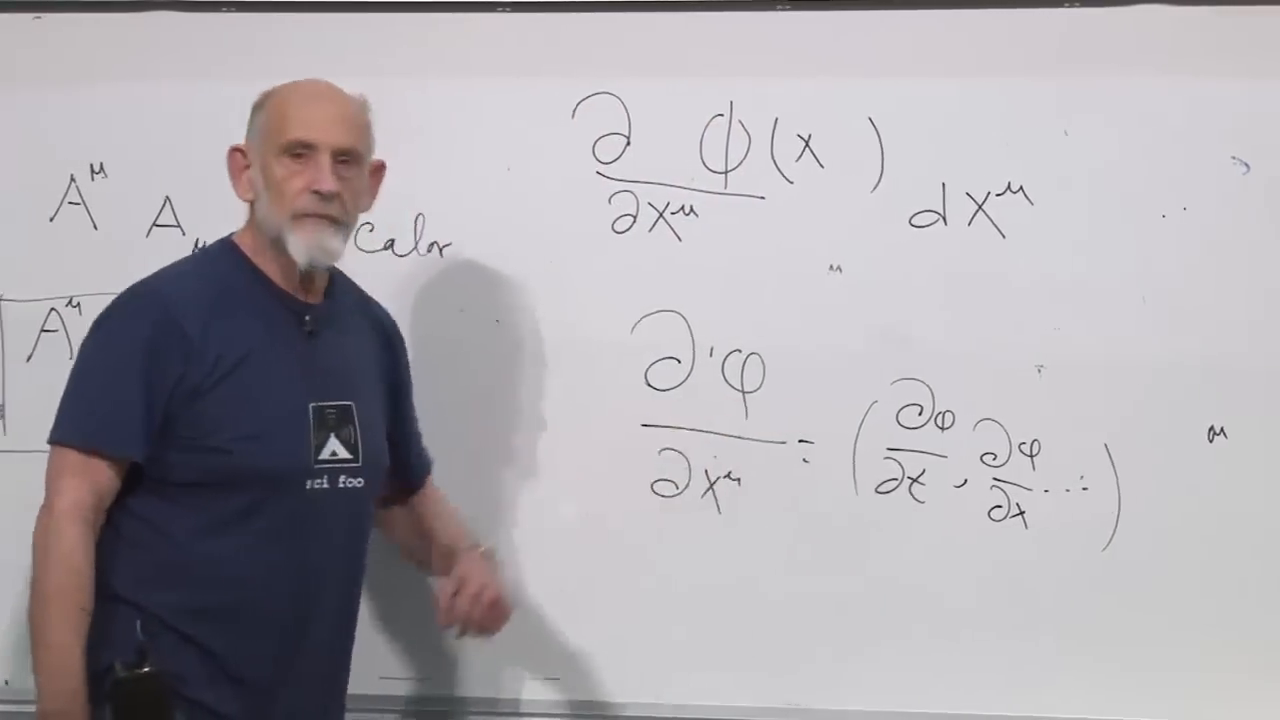
\includegraphics[width=0.90\textwidth]{lecture_05_figure_20.png}
\caption{微分\(d\phi=\partial_\mu\phi\,dx^\mu\)，标量梯度的余向量性质由此得出。}
\lectureframe{01:20:00}
\end{figure}

\begin{classroomqa}
\audiencequestion{\(x^\mu\)中的上指标在分母\(\partial/\partial x^\mu\)中出现时会变成下指标吗？}
\lecturerresponse{是的。坐标微分\(dx^\mu\)按逆变方式变换，因此它的对偶导数\(\partial_\mu=\partial/\partial x^\mu\)按协变方式变换。这正是使\(d\phi=\partial_\mu\phi\,dx^\mu\)成为标量的原因。\lecturetimestamp{01:20:00}}
\end{classroomqa}

\subsection{一个不变标量场密度}

将两个导数向量缩并：
\begin{align}
\partial_\mu\phi\,\partial^\mu\phi
&=
-(\partial_t\phi)^2
+(\partial_x\phi)^2
+(\partial_y\phi)^2
+(\partial_z\phi)^2.
\end{align}
因此自由标量密度可以紧凑地写成
\begin{equation}
\boxed{
\mathcal L_0
=
-\frac12
\partial_\mu\phi\,\partial^\mu\phi
}.
\label{eq:sr5-compact-density}
\end{equation}
这与\eqref{eq:sr5-free-field-action}中的分量密度完全相同。

\begin{figure}[htbp]
\centering
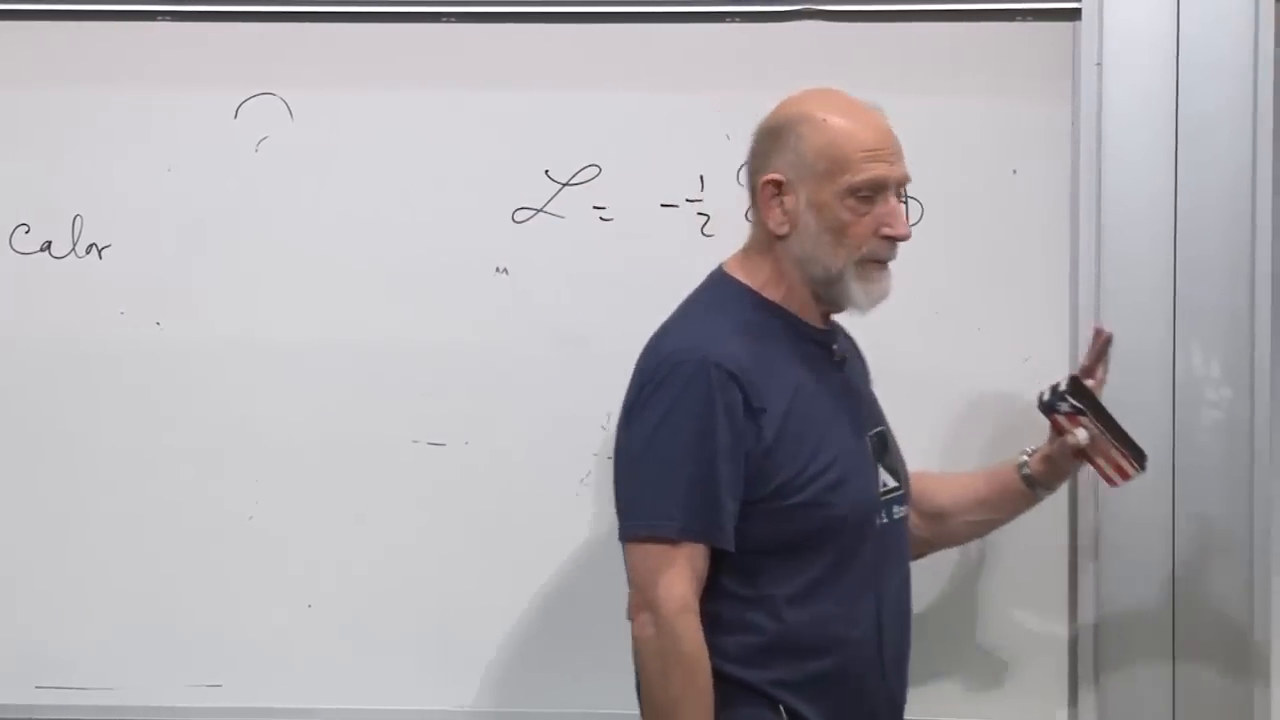
\includegraphics[width=0.90\textwidth]{lecture_05_figure_21.png}
\caption{标量场动能密度被浓缩为一个缩并表达式。}
\lectureframe{01:25:10}
\end{figure}

\begin{classroomqa}
\audiencequestion{这个缩并的一阶导数表达式是拉普拉斯算子吗？}
\lecturerresponse{不是。拉普拉斯算子包含二阶空间导数。这个表达式是拉格朗日密度，由一阶导数的乘积构成。\lecturetimestamp{01:24:38}}
\end{classroomqa}

标量密度在物理事件处的值与参考系无关。固有洛伦兹变换的行列式大小也为1，因此测度\(d^4x\)是不变的。 consequently，
\begin{equation}
S=\int d^4x\,\mathcal L
\end{equation}
是不变的。与参考系无关的作用量给出的欧拉--拉格朗日方程在每个惯性系中都具有相同形式。

\section{伽利略极限}

\begin{classroomqa}
\audiencequestion{牛顿力学中的拉格朗日量是否也必须遵循相对性原理？}
\lecturerresponse{是的，尽管此前并未强调这一点。牛顿方程在伽利略变换下不变，而伽利略变换是洛伦兹变换的\(c\to\infty\)极限。在该极限下消失的是同时性的相对性。\lecturetimestamp{01:27:16}}
\end{classroomqa}

为看出该极限，在沿\(x\)方向的推动中恢复\(c\)：
\begin{equation}
x'
=
\frac{x-vt}{\sqrt{1-v^2/c^2}},
\qquad
t'
=
\frac{t-vx/c^2}{\sqrt{1-v^2/c^2}}.
\label{eq:sr5-lorentz-c}
\end{equation}
取\(c\to\infty\)得到
\begin{equation}
\boxed{
x'=x-vt,
\qquad
t'=t
}.
\label{eq:sr5-galilean}
\end{equation}
这些就是伽利略变换。牛顿力学保留了相对性原理，即定律在所有惯性系中具有相同形式，但它同时也假定了一个为所有观察者所共有的绝对时间。

\begin{figure}[htbp]
\centering
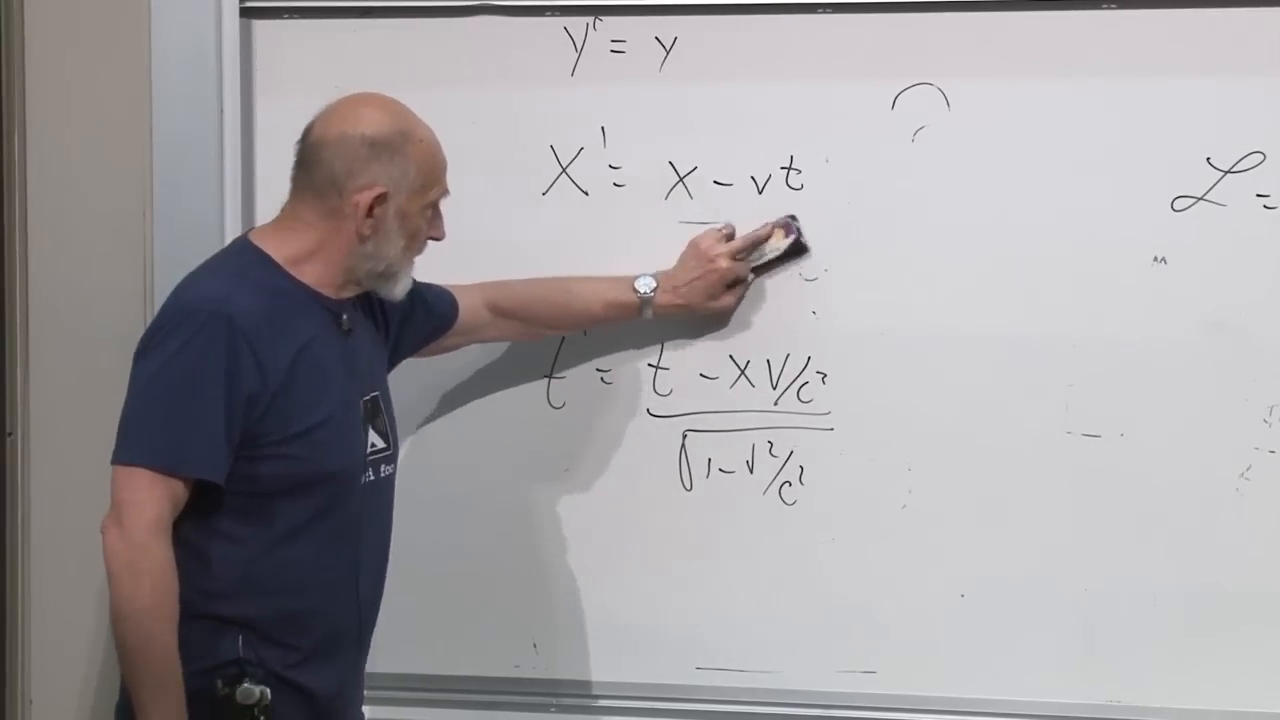
\includegraphics[width=0.90\textwidth]{lecture_05_figure_22.png}
\caption{取\(c\to\infty\)之前的洛伦兹推动，留下伽利略规则\(x'=x-vt\)和\(t'=t\)。}
\lectureframe{01:29:40}
\end{figure}

\begin{classroomqa}
\audiencequestion{上指标与下指标矢量是否仅相差一个符号变化？}
\lecturerresponse{对于此处所用的固定笛卡尔度规，对一个已知矢量降指标只改变其时间分量的符号。然而它们的洛伦兹变换法则是对偶法则，而不仅仅是一种任意的符号约定；度规才是将一种转换为另一种的东西。\lecturetimestamp{01:31:19}}
\end{classroomqa}

\begin{classroomqa}
\audiencequestion{坐标的每一个看似普通的函数都是标量吗？}
\lecturerresponse{不是。在每个坐标点处是一个数还不够；这个数必须在每个参考系中代表同一事件处的同一物理值。能量密度就是一个反例：推动一个盒子会同时改变所测得的能量和所测得的体积，因此观察者不会赋予相同的密度。\lecturetimestamp{01:33:23}}
\end{classroomqa}

四维速度的单个分量提供了另一个例子。完整的四维速度是一个矢量，但它的时间分量在推动下会改变，其本身并不是标量。

\section{克莱因--戈登场}

\subsection{谐振子的场类比}

回到标量密度并加上最简单的二次势：
\begin{equation}
\boxed{
\mathcal L
=
\frac12
\left[
(\partial_t\phi)^2
-|\boldsymbol{\nabla}\phi|^2
-\mu^2\phi^2
\right]
}.
\label{eq:sr5-kg-density}
\end{equation}
这是
\begin{equation}
L_{\mathrm{osc}}
=
\frac12\dot q^2-\frac12\mu^2q^2.
\end{equation}
的场论类比。每个空间点局部表现得像一个振子，而梯度项将相邻点耦合起来。

\begin{figure}[htbp]
\centering
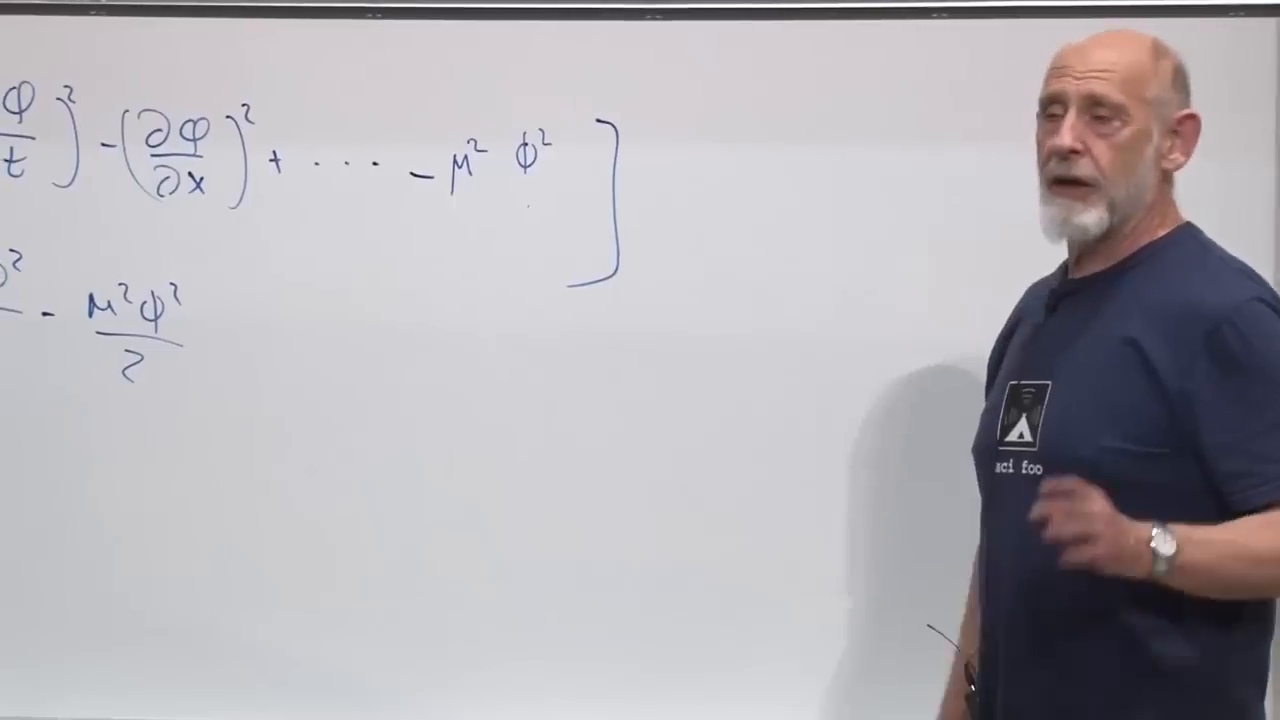
\includegraphics[width=0.90\textwidth]{lecture_05_figure_23.png}
\caption{二次标量场密度及其谐振子原型。}
\lectureframe{01:38:20}
\end{figure}

场的欧拉--拉格朗日方程为
\begin{equation}
\partial_\mu
\left[
\frac{\partial\mathcal L}
{\partial(\partial_\mu\phi)}
\right]
-
\frac{\partial\mathcal L}{\partial\phi}
=0.
\label{eq:sr5-field-el}
\end{equation}
将其应用于\eqref{eq:sr5-kg-density}得到
\begin{equation}
\boxed{
\partial_t^2\phi-\nabla^2\phi+\mu^2\phi=0
}.
\label{eq:sr5-kg}
\end{equation}
这就是克莱因--戈登方程。在主要为正号的约定下且
\(\Box=\partial_\mu\partial^\mu=-\partial_t^2+\nabla^2\)，同一方程为
\((\Box-\mu^2)\phi=0\)。

\begin{figure}[htbp]
\centering
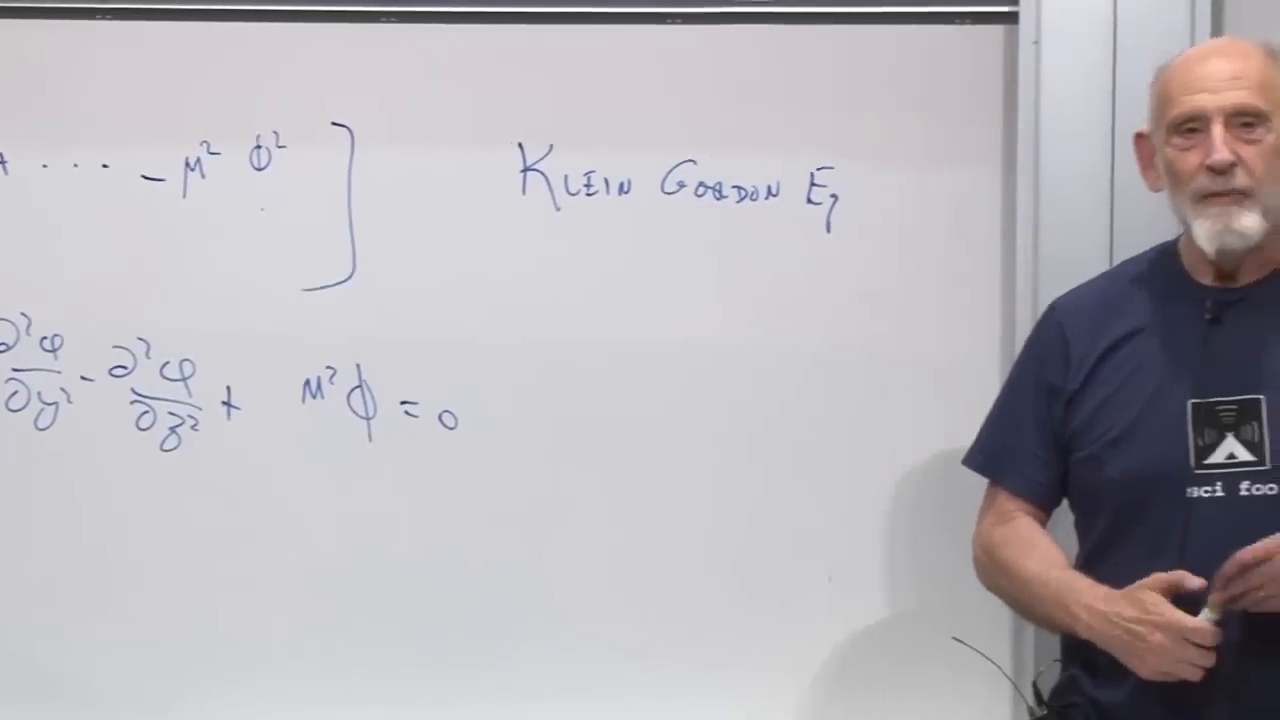
\includegraphics[width=0.90\textwidth]{lecture_05_figure_24.png}
\caption{克莱因--戈登方程被补写在它所由导出的密度下方。}
\lectureframe{01:40:00}
\end{figure}

历史上，该方程最初是作为相对论性单粒子波动方程来探讨的。那种解释遇到了困难，尤其是在正概率密度方面。它恰当的现代定位是相对论场论，在其中它支配自由标量场以及相互作用标量场的自由极限。

\subsection{平面波模式}

因为\eqref{eq:sr5-kg}是常系数线性方程，寻求平面波
\begin{equation}
\phi(x)
=
\exp\!\left[
-i\omega t+i\mathbf{k}\cdot\mathbf{x}
\right].
\label{eq:sr5-plane-wave}
\end{equation}
其中
\begin{equation}
k_\mu=(-\omega,k_x,k_y,k_z),
\end{equation}
指数为\(ik_\mu x^\mu\)。

\begin{figure}[htbp]
\centering
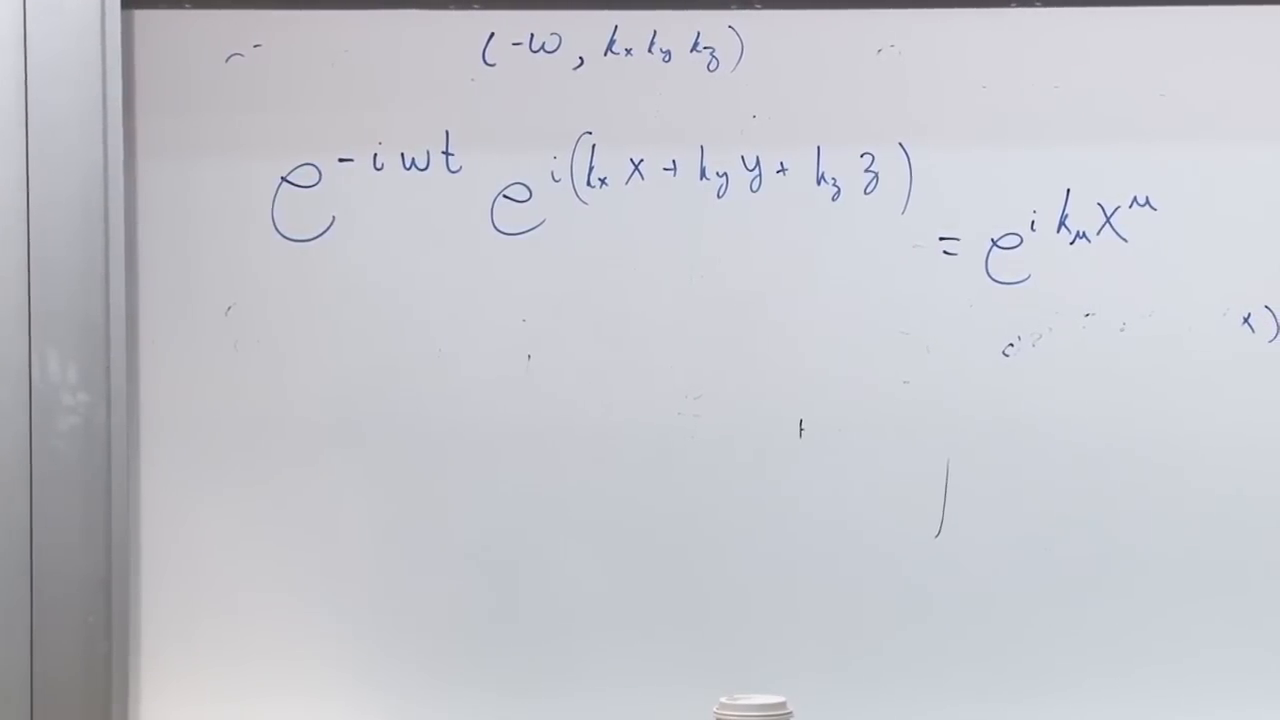
\includegraphics[width=0.90\textwidth]{lecture_05_figure_25.png}
\caption{平面波试探解按分量写出并写成\(e^{ik_\mu x^\mu}\)。}
\lectureframe{01:44:00}
\end{figure}

求导给出
\begin{equation}
\partial_t^2\phi=-\omega^2\phi,
\qquad
\nabla^2\phi=-|\mathbf{k}|^2\phi.
\end{equation}
代入\eqref{eq:sr5-kg}得到
\begin{equation}
\left(
-\omega^2+|\mathbf{k}|^2+\mu^2
\right)\phi=0.
\end{equation}
因此非零模式要求
\begin{equation}
\boxed{
\omega^2=|\mathbf{k}|^2+\mu^2
},
\qquad
\omega=\pm\sqrt{|\mathbf{k}|^2+\mu^2}.
\label{eq:sr5-dispersion}
\end{equation}

\begin{figure}[htbp]
\centering
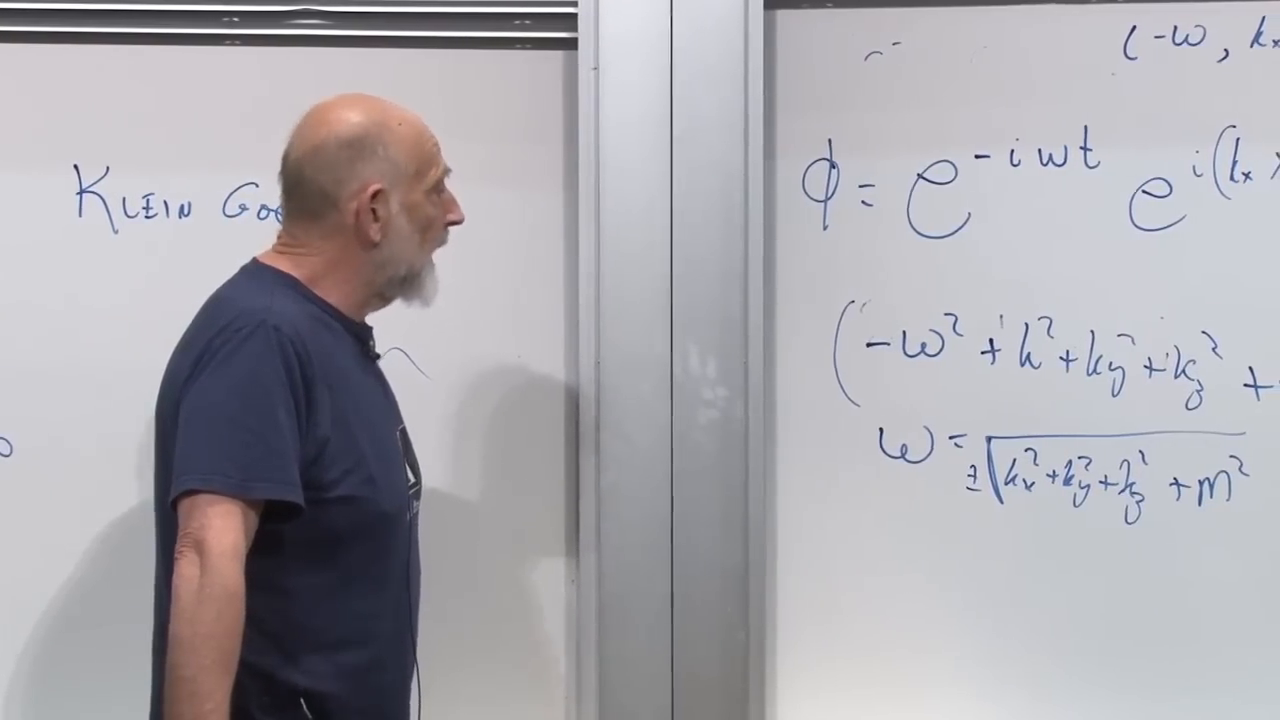
\includegraphics[width=0.90\textwidth]{lecture_05_figure_26.png}
\caption{平面波代入及由此得到的相对论色散关系。}
\lectureframe{01:47:00}
\end{figure}

在自然单位下，\(\mu\)起着质量的作用。对量子激发恢复常数，
\begin{equation}
E=\hbar\omega,
\qquad
\mathbf{p}=\hbar\mathbf{k},
\qquad
\mu=\frac{mc}{\hbar},
\end{equation}
将\eqref{eq:sr5-dispersion}变为
\begin{equation}
E^2=p^2c^2+m^2c^4.
\end{equation}
正频支和负频支都是经典解空间的一部分。通解是这些模式的叠加。

\begin{classroomqa}
\audiencequestion{克莱因--戈登方程从何而来？}
\lecturerresponse{它直接来自二次洛伦兹标量密度，通过场的欧拉--拉格朗日方程得到。选择这个例子是因为这个简单的二次密度产生一个线性场方程。\lecturetimestamp{01:47:59}}
\end{classroomqa}

\begin{classroomqa}
\audiencequestion{自然界中什么遵循克莱因--戈登方程？}
\lecturerresponse{自由经典标量场遵循。希格斯场涨落是标量的，在自由近似下约化为克莱因--戈登形式，尽管实际的希格斯场还具有相互作用和规范耦合。\lecturetimestamp{01:50:41}}
\end{classroomqa}

\section{标量背景作为质量移动}

现在粒子作用量重新回到视野中：
\begin{equation}
S_{\mathrm p}
=
-\int d\tau\,
\bigl[m+g\phi(x)\bigr].
\label{eq:sr5-final-particle-action}
\end{equation}
如果\(\phi\)具有恒定的背景值\(\phi_0\)，则粒子的运动就如同其质量为
\begin{equation}
\boxed{
m_{\mathrm{eff}}=m+g\phi_0
}.
\label{eq:sr5-effective-mass}
\end{equation}
如果裸项\(m\)消失，标量背景就可以提供乘以固有时所需的全部系数。

\begin{figure}[htbp]
\centering
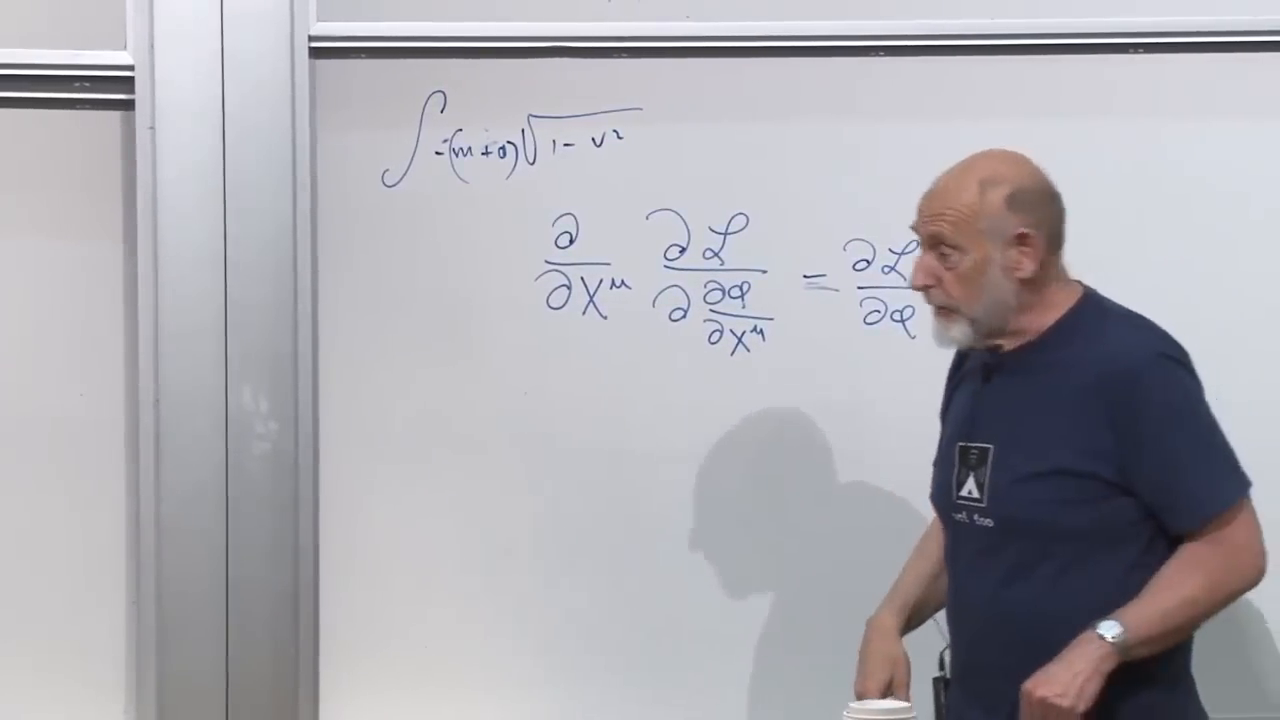
\includegraphics[width=0.90\textwidth]{lecture_05_figure_27.png}
\caption{上述依赖于场的粒子作用量满足紧致场欧拉--拉格朗日方程，从而将本讲的两部分内容联系起来。}
\lectureframe{01:51:30}
\end{figure}

这是一个刻意简化的希格斯质量产生模型。在标准模型中，费米子质量来自与希格斯真空期望值耦合的汤川耦合，示意性地为\(m_f\propto y_f v\)，而\(W\)和\(Z\)的质量则通过规范协变的希格斯动能项产生。玩具世界线耦合抓住了核心思想--非零的标量背景会改变惯性质量--但并不重现完整的电弱理论。此前建立的对偶关系仍然成立：将同一相互作用对场求变分，就会使粒子成为源。场作用于粒子，粒子也反过来作用于场。

\subsection{为什么复指数是有用的}

场不必在物理上是复的。欧拉公式给出
\begin{equation}
e^{i(\omega t-\mathbf{k}\cdot\mathbf{x})}
=
\cos(\omega t-\mathbf{k}\cdot\mathbf{x})
+i\sin(\omega t-\mathbf{k}\cdot\mathbf{x}).
\end{equation}
由于方程是实的且线性的，实部和虚部分别是实的解。它们是相差四分之一周期的波，而任何实线性组合仍然是解。

\begin{classroomqa}
\audiencequestion{当取实部时，虚部是否会以某种方式加为零？}
\lecturerresponse{不会。复指数将两个独立的实解——余弦和正弦——打包在一起。可以保留其中任一部分，也可以构成实的组合。之所以使用指数，是因为微分变成了乘法。\lecturetimestamp{01:53:29}}
\end{classroomqa}

\begin{figure}[htbp]
\centering
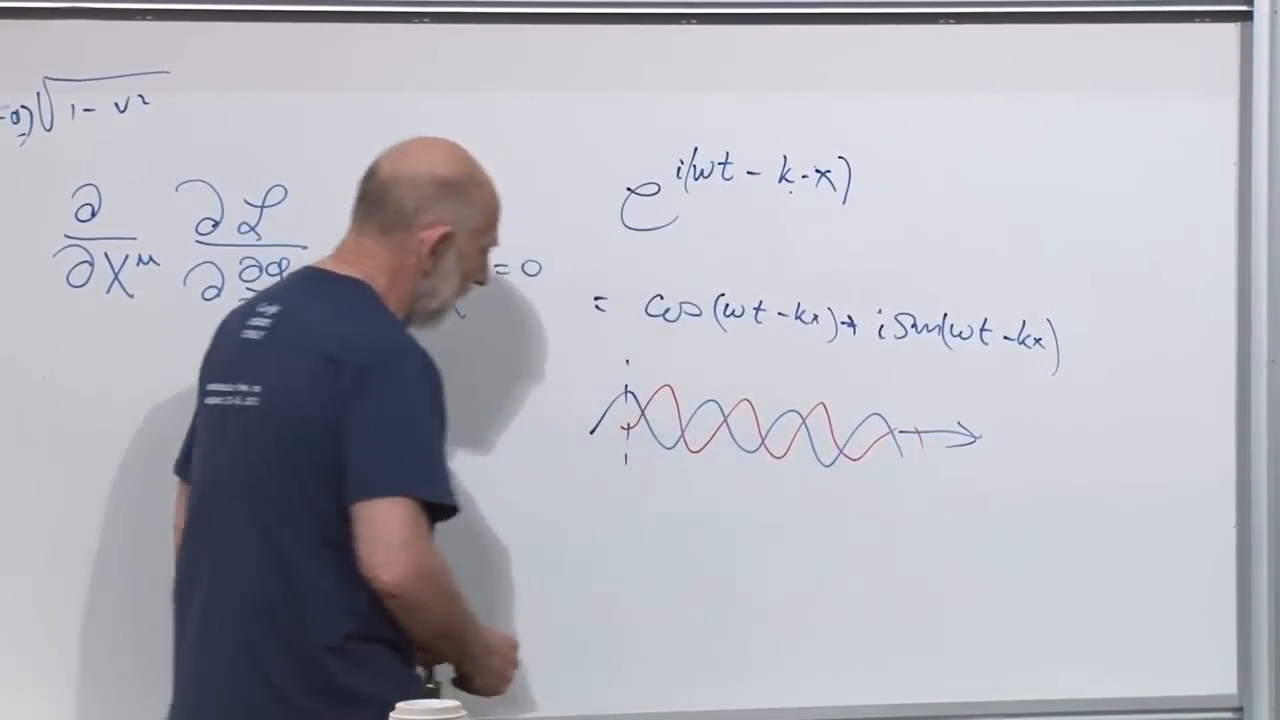
\includegraphics[width=0.90\textwidth]{lecture_05_figure_28.png}
\caption{一个复平面波被分解为余弦和正弦，画成两个相位不同的实波。}
\lectureframe{01:56:00}
\end{figure}

\begin{classroomqa}
\audiencequestion{超导体中电磁场获得质量是同一种现象吗？}
\lecturerresponse{它密切相关：在超导体中，凝聚体使电磁场在介质中获得有效质量，从而产生迈斯纳效应。完整的解释需要涉及电磁场，此处暂缓。\lecturetimestamp{01:56:14}}
\end{classroomqa}

\begin{classroomqa}
\audiencequestion{希格斯机制可以形象地理解为希格斯粒子在空间中飞行并分发质量吗？}
\lecturerresponse{不可以。相关的对象是希格斯场的背景值，而不是单个希格斯粒子的流。在玩具作用量中，背景只是改变了充当粒子质量的系数。\lecturetimestamp{01:57:31}}
\end{classroomqa}

\begin{classroomqa}
\audiencequestion{与同一标量背景的不同耦合会产生不同的质量吗？}
\lecturerresponse{会。移动量与耦合\(g\)成正比。在标准模型中，不同的汤川耦合正是不同费米子从同一希格斯背景获得不同质量的原因。\lecturetimestamp{01:58:04}}
\end{classroomqa}

\begin{classroomqa}
\audiencequestion{\(\phi\)本身就是质量项吗？}
\lecturerresponse{在这个玩具模型中，\(g\phi_0\)在一切力学意义上都充当对质量系数的贡献。耦合和背景值都必须包括在内。\lecturetimestamp{01:58:42}}
\end{classroomqa}

\begin{classroomqa}
\audiencequestion{如果希格斯背景消失，是否每个粒子都会变成无质量的？}
\lecturerresponse{不会。电子、夸克和弱规范玻色子将失去它们通常的电弱质量贡献，而中微子的细节取决于赋予中微子质量的机制。标量部门本身不必仅仅因为其背景值消失而变成无质量的。质子和中子的大部分质量反而来自QCD束缚和禁闭，因此并非直接由希格斯场产生。\lecturetimestamp{01:58:51}}
\end{classroomqa}

然而原子层面的后果是剧烈的。玻尔尺度表现为
\begin{equation}
a_0\sim\frac{1}{\alpha m_e}
\end{equation}
在自然单位制中。让电子质量趋于零会使通常的原子长度尺度发散；通常的局域原子将不复存在。质子和中子受到的影响则要间接得多，因为它们的质量主要是动力学QCD能量。

这些片段如今构成了一条连续的论证。洛伦兹几何支配着观测到的波长。一个作用量中的一个混合项使两个动力学系统相互影响。一个标量场既成为粒子的势，又成为由该粒子作为源的场。度规与指标记号使洛伦兹不变性变得可见，而最简单的二次不变密度则产生克莱因--戈尔登波。最后，一个恒定的标量背景将同一耦合转变为质量移动。贯穿始终的方法正是那个将持续下去的方法：构造一个不变作用量，对每一个动力学对象作变分，并从所得方程中读出相互作用的物理。